\documentclass[11pt]{article}
\usepackage{units}
\usepackage[small, bf]{caption}
\usepackage[numbers,sort&compress]{natbib}
\usepackage{color}
\usepackage{amssymb, amsmath}
\usepackage{graphicx}
\usepackage{epstopdf}
\usepackage{verbatim}
\usepackage{amsfonts}
\usepackage{subfloat}
\usepackage{subfig}
\usepackage{multirow}
\usepackage{authblk}
\usepackage{array}
\usepackage{footmisc}
\usepackage{tabularx}
\usepackage{sidecap}
\usepackage{setspace}
\usepackage[normalem]{ulem}
\usepackage{pgfplotstable}
\usepackage[margin=1in]{geometry}
\renewcommand\Affilfont{\small}
\newcommand{\ignore}[1]{}
\usepackage{float}

\newenvironment{packed_enum}{
\begin{enumerate}
  \setlength{\itemsep}{1pt}
  \setlength{\parskip}{0pt}
  \setlength{\parsep}{0pt}
}{\end{enumerate}}
\newenvironment{packed_itemize}{
\begin{itemize}
  \setlength{\itemsep}{1pt}
  \setlength{\parskip}{0pt}
  \setlength{\parsep}{0pt}
}{\end{itemize}}
\newenvironment{packed_desc}{
\begin{description}
  \setlength{\itemsep}{1pt}
  \setlength{\parskip}{0pt}
  \setlength{\parsep}{0pt}
}{\end{description}}

\def\AI#1{{\textcolor{red}{#1}}}
\def\dHAF{\text{-HAF}}
\def\HAF{\text{HAF}}
\def\HAFpeak{\text{HAF-peak}}
\def\HAFtrough{\text{HAF-trough}}
\def\HAFneutral{\text{HAF}_{\text{neutral}}}
\def\TMRCA{T_{\text{MRCA}}}

\def\VB#1{{\textcolor{blue}{VB note: #1}}}

\newcommand{\algoname}{\ensuremath{\text{PreCIOSS}}}
\def\vecbold#1{{\boldsymbol#1}}

%%%%%%%%%%%%
\makeatletter
\renewcommand\section{\@startsection {section}{1}{\z@}%                                                                                                         
                                   {-3.2ex \@plus -1ex \@minus -.2ex}%                                                                                        
                                   {2.0ex \@plus.2ex}%                                                                                                        
                                   {\normalfont\Large\bfseries}}
\renewcommand\subsection{\@startsection{subsection}{2}{\z@}%                                                                                                    
                                     {-2.95ex\@plus -1ex \@minus -.2ex}%                                                                                      
                                     {1.2ex \@plus .2ex}%                                                                                                     
                                     {\normalfont\large\bfseries}}
\renewcommand\subsubsection{\@startsection{subsubsection}{3}{\z@}%                                                                                              
                                     {-2.95ex\@plus -1ex \@minus -.2ex}%                                                                                      
                                     {1.2ex \@plus .2ex}%                                                                                                     
                                     {\normalfont\normalsize\bfseries}}
\renewcommand\paragraph{\@startsection{paragraph}{4}{\z@}%                                                                                                      
                                    {1.55ex \@plus1ex \@minus.2ex}%                                                                                           
                                    {-.7em}%                                                                                                                   
                                    {\normalfont\normalsize\bfseries}}
\makeatother
%%%%%%%%%%%%%%%%% Arya's
\usepackage{color,hyperref}
\hypersetup{colorlinks,breaklinks,linkcolor=darkblue,urlcolor=darkblue, anchorcolor=darkblue,citecolor=darkblue}
\usepackage{amssymb,amsmath,amsthm,amsfonts}
\usepackage{mathtools}
\usepackage{enumerate}
\definecolor{darkgreen}{rgb}{0,0.55,0}
\definecolor{orange}{rgb}{1,0.55,0}
\definecolor{darkblue}{rgb}{0.0,0.0,0.5}
\def\Arya#1{{\textcolor{darkgreen}{Arya note: #1}}}
\def\emphr#1{{\textcolor{red}{#1}}}
\def\emphg#1{{\textcolor{darkgreen}{#1}}}
\def\emphb#1{{\textcolor{darkblue}{#1}}}
\usepackage{pifont}
\newcommand{\cmark}{\ding{51}}%
\newcommand{\xmark}{\ding{55}}%
\usepackage{bbm}
\def\datadm{data from a study of \dmel adaptation to alternating temperatures}
\def\comale{\text{{\sc Clear}}}
\newcommand{\dataset}{{\cal D}}
\newcommand{\fracpartial}[2]{\frac{\partial #1}{\partial  #2}}
\newcommand{\phibp}{\phi_{ \hspace{-0.025in}\scalebox{.45}{\text{ BP}}}}
\newcommand{\phics}{\phi_{ \hspace{-0.025in}\scalebox{.45}{\text{ CS}}}}
\newcommand{\lone}{$\ell_1$-norm }
%\def\lll{\mbox{\ell_1}}
\def\dmel{\emph{D. melanogaster }}

\DeclareMathOperator{\tw}{tw}
\DeclareMathOperator{\local}{local}
\DeclareMathOperator{\range}{range}
\DeclareMathOperator{\Path}{Path}
\DeclareMathOperator{\Sg}{Sg}
\DeclareMathOperator{\spt}{SP}
\DeclareMathOperator{\avg}{avg}
\DeclareMathOperator{\nbd}{\mathcal{N}}
\DeclareMathOperator{\parent}{Pa}
\DeclareMathOperator{\Cq}{Cq}
\DeclareMathOperator{\TW}{TW}
\DeclareMathOperator{\approxML}{ApproxML}
\DeclareMathOperator{\Bethe}{Bethe}
\DeclareMathOperator{\TRW}{TRW}
\DeclareMathOperator{\conv}{Conv}
\DeclareMathOperator{\dir}{Dir}
\DeclareMathOperator{\mult}{Mult}
\DeclareMathOperator{\cat}{Cat}
\DeclareMathOperator{\crp}{CRP(\gamma)}
\DeclareMathOperator{\ncrp}{nCRP}
\DeclareMathOperator{\node}{node}
\DeclareMathOperator{\nodes}{nodes}
\DeclareMathOperator{\pr}{Pr}
\DeclareMathOperator{\dom}{\bf Dom}
\DeclareMathOperator{\lbp}{LBP}
\DeclareMathOperator{\Corr}{Corr}
\DeclareMathOperator{\hCorr}{\widehat{Corr}}
\DeclareMathOperator{\hSc}{\widehat{\mathcal{S}}}
\DeclareMathOperator{\tr}{Tr}
\DeclareMathOperator{\mst}{MST}
\DeclareMathOperator{\supp}{Supp}
\DeclareMathOperator{\dtv}{d_{TV}}
\DeclareMathOperator{\hdtv}{\hd_{TV}}
\DeclareMathOperator*{\argmin}{arg\,min}
\DeclareMathOperator*{\argmax}{arg\,max}
\DeclareMathOperator*{\esssup}{ess\,sup}
\DeclareMathOperator*{\essinf}{ess\,inf}
\DeclareMathOperator{\dist}{dist}
\DeclareMathOperator{\rank}{Rank}
\DeclareMathOperator{\Krank}{Rank_K}
\DeclareMathOperator{\Det}{Det}
\DeclareMathOperator{\poiss}{Poiss}
\DeclareMathOperator{\unif}{Unif} \DeclareMathOperator{\Deg}{Deg}
\def\simiid{{\overset{i.i.d.}{\sim}}}
\def\lcv{{\,\,\underset{cv}{\leq}\,\,}}
\def\gcv{{\,\,\underset{cv}{\geq}\,\,}}
\def\lcx{{\,\,\underset{cx}{\leq}\,\,}}
\def\gcx{{\,\,\underset{cx}{\geq}\,\,}}
\def\leqst{{\,\,\overset{st}{\leq}\,\,}}
\def\geqst{{\,\,\overset{st}{\geq}\,\,}}
\def\eqdist{{\,\,\overset{d}{=}\,\,}}
\def\geqrh{{\,\,\overset{rh}{\geq}\,\,}}
\def\geqlr{{\,\,\overset{lr}{\geq}\,\,}}
\def\eqlr{{\,\,\overset{lr}{=}\,\,}}
\def\tha{{\mbox{\tiny th}}}

\DeclareMathOperator{\Aug}{Aug}
\DeclareMathOperator{\watts}{Watts}
\DeclareMathOperator{\girth}{Girth}
\DeclareMathOperator{\PL}{PL}
\DeclareMathOperator{\LP}{LP}
\DeclareMathOperator{\ER}{ER}
\DeclareMathOperator{\reg}{Reg}
\DeclareMathOperator{\Var}{Var}
\DeclareMathOperator{\hSigma}{\widehat{\Sigma}}
\DeclareMathOperator{\Cov}{Cov}
\DeclareMathOperator{\Poiss}{Poiss}
\DeclareMathOperator{\Diag}{Diag}
\DeclareMathOperator{\Diam}{Diam}
\def\erf{\mbox{erf}}
\def\erfc{\mbox{erfc}}
\def\qfunc{\mbox{Q}}
%\def\myexp{\mbox{e}}
\def\snr{\mbox{{SNR}}}
\def\signum{\mbox{sgn}}
\def\Card{\mbox{Card}}
\DeclareMathOperator*{\plim}{plim}
\def\convd{\overset{d}\rightarrow}
\def\convp{\overset{p}\rightarrow}
\newcommand\indep{\protect\mathpalette{\protect\independenT}{\perp}}
\def\independenT#1#2{\mathrel{\rlap{$#1#2$}\mkern2mu{#1#2}}}
\def\pl{{\parallel}}
\DeclarePairedDelimiter\norm{\lVert}{\rVert}
\DeclarePairedDelimiter\nuclearnorm{\lVert}{\rVert_*}
\DeclarePairedDelimiter\onenorm{\lVert}{\rVert_1}
\DeclarePairedDelimiter\znorm{\lVert}{\rVert_0}
\def\rinfnorm{\rVert_{\infty}}
\DeclarePairedDelimiter\infnorm{\lVert}{\rinfnorm}
\def\lnorm{{\lvert\!\lvert\!\lvert}}
\def\rnorm{{\rvert\!\rvert\!\rvert}}
\DeclarePairedDelimiter\gennorm{\lnorm}{\rnorm}
 \DeclarePairedDelimiter\abs{\lvert}{\rvert}
 \DeclarePairedDelimiter\geninfnorm{\lnorm}{\rnorm_{\infty}}
 \DeclarePairedDelimiter\genonenorm{\lnorm}{\rnorm_{1}}
\DeclareMathOperator{\atanh}{atanh}
 \DeclareMathOperator{\sech}{sech}
 \def\0{{\bf 0}}

\DeclareMathOperator{\lea}{\overset{(a)}{\leq}}
\DeclareMathOperator{\leb}{\overset{(b)}{\leq}}
\DeclareMathOperator{\lec}{\overset{(c)}{\leq}}
\DeclareMathOperator{\led}{\overset{(d)}{\leq}}
\DeclareMathOperator{\lee}{\overset{(e)}{\leq}}

\DeclareMathOperator{\eqa}{\overset{(a)}{=}}
\DeclareMathOperator{\eqb}{\overset{(b)}{=}}
\DeclareMathOperator{\eqc}{\overset{(c)}{=}}
\DeclareMathOperator{\eqd}{\overset{(d)}{=}}
\DeclareMathOperator{\eqe}{\overset{(e)}{=}}

\DeclareMathOperator{\gea}{\overset{(a)}{\geq}}
\DeclareMathOperator{\geb}{\overset{(b)}{\geq}}
\DeclareMathOperator{\gec}{\overset{(c)}{\geq}}
\DeclareMathOperator{\ged}{\overset{(d)}{\geq}}
\DeclareMathOperator{\gee}{\overset{(e)}{\geq}}

\def\viz{{viz.,\ \/}}
\def\ie{{i.e.,\ \/}}
\def\eg{{e.g.,\ \/}}
\def\etc{{etc.  }}
\def\ifff{{iff  }}
\def\as{{a.s.  }}
\def\st{{s.t.  }}
\def\wpone{{w.p.}\,1\,\,}
\def\wpp{{w.p.p.}\,\,}
\def\for{\,\,\mbox{for}\quad}
\def\ifmbox{\,\,\mbox{if}\quad}
\def\nn{\nonumber}
%\def\qed{\hfill$\Box$}

\def\qed{\hfill\hbox{${\vcenter{\vbox{
    \hrule height 0.4pt\hbox{\vrule width 0.4pt height 6pt
    \kern5pt\vrule width 0.4pt}\hrule height 0.4pt}}}$}}
\def\complx{\mathbb{C}}

%%%%%%%%%%%%%%%%%%%%%%%%%%%%%%%%%%%%%%%%%%%%%%%%%%%%%%%%%%%%% Color

\def\tcr{\textcolor{red}}
\def\tcb{\textcolor{blue}}
\def\tcg{\textcolor{green}}
\def\tcw{\textcolor{white}}
\def\tcm{\textcolor{magenta}}
\def\tccyan{\textcolor{cyan}}
\def\tcv{\textcolor{violet}}
\definecolor{myred}{rgb}{0.3,0.0,0.7}
\definecolor{dkg}{rgb}{0.1,0.7,0.2}
\definecolor{dkb}{rgb}{0.0,0.2,0.8}

\def\tcdkb{\textcolor{dkb}}
\def\tcdkg{\textcolor{dkg}}


%%%%%%%%%%%%%%%%%%%%%%%%%%%%%%%%%%%%%%%%%%%%%%%%%%%%%%%%%%%%%
\newcommand{\Amsc}{\mathscr{A}}
\newcommand{\Cmsc}{\mathscr{C}}
\newcommand{\Dmsc}{\mathscr{D}}
\newcommand{\Emsc}{\mathscr{E}}
\newcommand{\Fmsc}{\mathscr{F}}
\newcommand{\Gmsc}{\mathscr{G}}
\newcommand{\Hmsc}{\mathscr{H}}
\newcommand{\Kmsc}{\mathscr{K}}
\newcommand{\Nmsc}{\mathscr{N}}
\newcommand{\Pmsc}{\mathscr{P}}
\newcommand{\Qmsc}{\mathscr{Q}}
\newcommand{\Rmsc}{\mathscr{R}}
\newcommand{\Smsc}{\mathscr{S}}
\newcommand{\Tmsc}{\mathscr{T}}
\newcommand{\Umsc}{\mathscr{U}}
\newcommand{\Xmsc}{\mathscr{X}}
\newcommand{\Ymsc}{\mathscr{Y}}

%%%%%%%%%%%%%%%%%%%%%%%%%%%%%%%%%%%%%%%%%%%%%%%%%%%%%%%%%%%%% Hat
\def\ha{\widehat{a}}
\def\hb{\widehat{b}}
\def\hc{\widehat{c}}
\def\hd{\widehat{d}}
\def\he{\widehat{e}}
\def\hf{\widehat{f}}
\def\hg{\widehat{g}}
\def\hh{\widehat{h}}
\def\hi{\widehat{i}}
\def\hj{\widehat{j}}
\def\hk{\widehat{k}}
\def\hl{\widehat{l}}
\def\hm{\widehat{m}}
\def\hn{\widehat{n}}
\def\ho{\widehat{o}}
\def\hp{\widehat{p}}
\def\hq{\widehat{q}}
\def\hr{\widehat{r}}
\def\hs{\widehat{s}}
\def\hatt{\widehat{t}}
\def\hu{\widehat{u}}
\def\hv{\widehat{v}}
\def\hw{\widehat{w}}
\def\hx{\widehat{x}}
\def\hy{\widehat{y}}
\def\hz{\widehat{z}}

\def\hA{\widehat{A}}
\def\hB{\widehat{B}}
\def\hC{\widehat{C}}
\def\hD{\widehat{D}}
\def\hE{\widehat{E}}
\def\hF{\widehat{F}}
\def\hG{\widehat{G}}
\def\hH{\widehat{H}}
\def\hI{\widehat{I}}
\def\hJ{\widehat{J}}
\def\hK{\widehat{K}}
\def\hL{\widehat{L}}
\def\hM{\widehat{M}}
\def\hN{\widehat{N}}
\def\hO{\widehat{O}}
\def\hP{\widehat{P}}
\def\hQ{\widehat{Q}}
\def\hR{\widehat{R}}
\def\hS{\widehat{S}}
\def\hT{\widehat{T}}
\def\hU{\widehat{U}}
\def\hV{\widehat{V}}
\def\hW{\widehat{W}}
\def\hX{\widehat{X}}
\def\hY{\widehat{Y}}
\def\hZ{\widehat{Z}}
\def\hlambda{\widehat{\lambda}}
\def\hpi{\widehat{\pi}}
\def\hnu{\widehat{\nu}}
\def\hbd{\widehat{\mathbf{d}}}
\def\bLambda{\mathbf{\Lambda}}


%%%%%%%%%%%%%%%%%%%%%%%%%%%%%%%%%%%%%%%%%%%%%%%%%%%%%%%%%%%%% Vector
\def\valpha{\vec{\alpha}}
\def\va{\vec{a}}
\def\vb{\vec{b}}
\def\vc{\vec{c}}
\def\vd{\vec{d}}
\def\ve{\vec{e}}
\def\vf{\vec{f}}
\def\vg{\vec{g}}
\def\vh{\vec{h}}
\def\vi{\vec{i}}
\def\vj{\vec{j}}
\def\vk{\vec{k}}
\def\vl{\vec{l}}
\def\vm{\vec{m}}
\def\vn{\vec{n}}
\def\vo{\vec{o}}
\def\vp{\vec{p}}
\def\vq{\vec{q}}
\def\vr{\vec{r}}
\def\vs{\vec{s}}
\def\vt{\vec{t}}
\def\vu{\vec{u}}
\def\vv{\vec{v}}
\def\vw{\vec{w}}
\def\vx{\vec{x}}
\def\vy{\vec{y}}
\def\vz{\vec{z}}

\def\vA{\vec{A}}
\def\vB{\vec{B}}
\def\vC{\vec{C}}
\def\vD{\vec{D}}
\def\vE{\vec{E}}
\def\vF{\vec{F}}
\def\vG{\vec{G}}
\def\vH{\vec{H}}
\def\vI{\vec{I}}
\def\vJ{\vec{J}}
\def\vK{\vec{K}}
\def\vL{\vec{L}}
\def\vM{\vec{M}}
\def\vN{\vec{N}}
\def\vO{\vec{O}}
\def\vP{\vec{P}}
\def\vQ{\vec{Q}}
\def\vR{\vec{R}}
\def\vS{\vec{S}}
\def\vT{\vec{T}}
\def\vU{\vec{U}}
\def\vV{\vec{V}}
\def\vW{\vec{W}}
\def\vX{\vec{X}}
\def\vY{\vec{Y}}
\def\vZ{\vec{Z}}

%%%%%%%%%%%%%%%%%%%%%%%%%%%%%%%%%%%%%%%%%%%%%%%%%%%%%%%%%%%%% Bold
\def\bfalpha{{\boldsymbol {\alpha}}}
\def\bfnu{{\boldsymbol {\nu}}}
\def\bfeta{{\boldsymbol {\eta}}}
\def\bfzero{{\mathbf{0}}}
\def\bfone{{\mathbf{1}}}
\def\bfa{{\mathbf a}}
\def\bfb{{\mathbf b}}
\def\bfc{{\mathbf c}}
\def\bfd{{\mathbf d}}
\def\bfe{{\mathbf e}}
\def\bff{{\mathbf f}}
\def\bfg{{\mathbf g}}
\def\bfh{{\mathbf h}}
\def\bfi{{\mathbf i}}
\def\bfj{{\mathbf j}}
\def\bfk{{\mathbf k}}
\def\bfl{{\mathbf l}}
\def\bfm{{\mathbf m}}
\def\bfn{{\mathbf n}}
\def\bfo{{\mathbf o}}
\def\bfp{{\mathbf p}}
\def\bfq{{\mathbf q}}
\def\bfr{{\mathbf r}}
\def\bfs{{\mathbf s}}
\def\bft{{\mathbf t}}
\def\bfu{{\mathbf u}}
\def\bfv{{\mathbf v}}
\def\bfw{{\mathbf w}}
\def\bfx{{\mathbf x}}
\def\bfy{{\mathbf y}}
\def\bfz{{\mathbf z}}

\def\bfA{{\mathbf A}}
\def\bfB{{\mathbf B}}
\def\bfC{{\mathbf C}}
\def\bfD{{\mathbf D}}
\def\bfE{{\mathbf E}}
\def\bfF{{\mathbf F}}
\def\bfG{{\mathbf G}}
\def\bfH{{\mathbf H}}
\def\bfI{{\mathbf I}}
\def\bfJ{{\mathbf J}}
\def\bfK{{\mathbf K}}
\def\bfL{{\mathbf L}}
\def\bfM{{\mathbf M}}
\def\bfN{{\mathbf N}}
\def\bfO{{\mathbf O}}
\def\bfP{{\mathbf P}}
\def\bfQ{{\mathbf Q}}
\def\bfR{{\mathbf R}}
\def\bfS{{\mathbf S}}
\def\bfT{{\mathbf T}}
\def\bfU{{\mathbf U}}
\def\bfV{{\mathbf V}}
\def\bfW{{\mathbf W}}
\def\bfX{{\mathbf X}}
\def\bfY{{\mathbf Y}}
\def\bfZ{{\mathbf Z}}


%%%%%%%%%%%%%%%%%%%%%%%%%%%%%%%%%%%%%%%%%%%%%%%%%%%%%%%%%%%%% Bold Symbols
\def\alphabf{\hbox{\boldmath$\alpha$\unboldmath}}
\def\betabf{\hbox{\boldmath$\beta$\unboldmath}}
\def\gammabf{\hbox{\boldmath$\gamma$\unboldmath}}
\def\deltabf{\hbox{\boldmath$\delta$\unboldmath}}
\def\epsilonbf{\hbox{\boldmath$\epsilon$\unboldmath}}
\def\zetabf{\hbox{\boldmath$\zeta$\unboldmath}}
\def\etabf{\hbox{\boldmath$\eta$\unboldmath}}
\def\iotabf{\hbox{\boldmath$\iota$\unboldmath}}
\def\kappabf{\hbox{\boldmath$\kappa$\unboldmath}}
\def\lambdabf{\hbox{\boldmath$\lambda$\unboldmath}}
\def\mubf{\hbox{\boldmath$\mu$\unboldmath}}
\def\nubf{\hbox{\boldmath$\nu$\unboldmath}}
\def\xibf{\hbox{\boldmath$\xi$\unboldmath}}
\def\pibf{\hbox{\boldmath$\pi$\unboldmath}}
\def\rhobf{\hbox{\boldmath$\rho$\unboldmath}}
\def\sigmabf{\hbox{\boldmath$\sigma$\unboldmath}}
\def\taubf{\hbox{\boldmath$\tau$\unboldmath}}
\def\upsilonbf{\hbox{\boldmath$\upsilon$\unboldmath}}
\def\phibf{\hbox{\boldmath$\phi$\unboldmath}}
\def\chibf{\hbox{\boldmath$\chi$\unboldmath}}
\def\psibf{\hbox{\boldmath$\psi$\unboldmath}}
\def\omegabf{\hbox{\boldmath$\omega$\unboldmath}}
\def\inftybf{\hbox{\boldmath$\infty$\unboldmath}}
\def\hSigmabf{\hbox{$\widehat{\bf \Sigma}$}}
\def\Sigmabf{\hbox{$\bf \Sigma$}}
\def\Upsilonbf{\hbox{$\bf \Upsilon$}}
\def\Omegabf{\hbox{$\bf \Omega$}}
\def\Deltabf{\hbox{$\bf \Delta$}}
\def\Gammabf{\hbox{$\bf \Gamma$}}
\def\Thetabf{\hbox{$\bf \Theta$}}
\def\Lambdabf{\mbox{$ \bf \Lambda $}}
\def\Xibf{\hbox{\bf$\Xi$}}
\def\Pibf{{\bf \Pi}}
\def\thetabf{{\mbox{\boldmath$\theta$\unboldmath}}}
\def\Upsilonbf{\hbox{\boldmath$\Upsilon$\unboldmath}}
\newcommand{\Phibf}{\mbox{${\bf \Phi}$}}
\newcommand{\Psibf}{\mbox{${\bf \Psi}$}}
\def\olambda{\mathfrak{o}(\lambda)}
\def\complex{\mathfrak{C}}

%%%%%%%%%%%%%%%%%%%%%%%%%%%%%%%%%%%%%%%%%%%%%%%%%%%%%%%%%%%%% Bar
\def\brzero{{\overline{{0}}}}
\def\brone{{\overline{{1}}}}
\def\bra{{\overline{a}}}
\def\brb{{\overline{b}}}
\def\brc{{\overline{c}}}
\def\brd{{\overline{d}}}
\def\bre{{\overline{e}}}
\def\brf{{\overline{f}}}
\def\brg{{\overline{g}}}
\def\brh{{\overline{h}}}
\def\bri{{\overline{i}}}
\def\brj{{\overline{j}}}
\def\brk{{\overline{k}}}
\def\brl{{\overline{l}}}
\def\brm{{\overline{m}}}
\def\brn{{\overline{n}}}
\def\bro{{\overline{o}}}
\def\brp{{\overline{p}}}
\def\brq{{\overline{q}}}
\def\brr{{\overline{r}}}
\def\brs{{\overline{s}}}
\def\brt{{\overline{t}}}
\def\bru{{\overline{u}}}
\def\brv{{\overline{v}}}
\def\brw{{\overline{w}}}
\def\brx{{\overline{x}}}
\def\bry{{\overline{y}}}
\def\brz{{\overline{z}}}

\def\brA{{\overline{A}}}
\def\brB{{\overline{B}}}
\def\brC{{\overline{C}}}
\def\brD{{\overline{D}}}
\def\brE{{\overline{E}}}
\def\brF{{\overline{F}}}
\def\brG{{\overline{G}}}
\def\brH{{\overline{H}}}
\def\brI{{\overline{I}}}
\def\brJ{{\overline{J}}}
\def\brK{{\overline{K}}}
\def\brL{{\overline{L}}}
\def\brM{{\overline{M}}}
\def\brN{{\overline{N}}}
\def\brO{{\overline{O}}}
\def\brP{{\overline{P}}}
\def\brQ{{\overline{Q}}}
\def\brR{{\overline{R}}}
\def\brS{{\overline{S}}}
\def\brT{{\overline{T}}}
\def\brU{{\overline{U}}}
\def\brV{{\overline{V}}}
\def\brW{{\overline{W}}}
\def\brX{{\overline{X}}}
\def\brY{{\overline{Y}}}
\def\beZ{{\overline{Z}}}

%%%%%%%%%%%%%%%%%%%%%%%%%%%%%%%%%%%%%%%%%%%%%%%%%%%%%%%%%%%%% Bar Bold 
\def\bbfzero{{\overline{\mathbf{0}}}}
\def\bbfone{{\overline{\mathbf{1}}}}
\def\bbfa{{\overline{\mathbf a}}}
\def\bbfb{{\overline{\mathbf b}}}
\def\bbfc{{\overline{\mathbf c}}}
\def\bbfd{{\overline{\mathbf d}}}
\def\bbfe{{\overline{\mathbf e}}}
\def\bbff{{\overline{\mathbf f}}}
\def\bbfg{{\overline{\mathbf g}}}
\def\bbfh{{\overline{\mathbf h}}}
\def\bbfi{{\overline{\mathbf i}}}
\def\bbfj{{\overline{\mathbf j}}}
\def\bbfk{{\overline{\mathbf k}}}
\def\bbfl{{\overline{\mathbf l}}}
\def\bbfm{{\overline{\mathbf m}}}
\def\bbfn{{\overline{\mathbf n}}}
\def\bbfo{{\overline{\mathbf o}}}
\def\bbfp{{\overline{\mathbf p}}}
\def\bbfq{{\overline{\mathbf q}}}
\def\bbfr{{\overline{\mathbf r}}}
\def\bbfs{{\overline{\mathbf s}}}
\def\bbft{{\overline{\mathbf t}}}
\def\bbfu{{\overline{\mathbf u}}}
\def\bbfv{{\overline{\mathbf v}}}
\def\bbfw{{\overline{\mathbf w}}}
\def\bbfx{{\overline{\mathbf x}}}
\def\bbfy{{\overline{\mathbf y}}}
\def\bbfz{{\overline{\mathbf z}}}

\def\bbfA{{\overline{\mathbf A}}}
\def\bbfB{{\overline{\mathbf B}}}
\def\bbfC{{\overline{\mathbf{C}}}}
\def\bbfD{{\overline{\mathbf D}}}
\def\bbfE{{\overline{\mathbf E}}}
\def\bbfF{{\overline{\mathbf F}}}
\def\bbfG{{\overline{\mathbf G}}}
\def\bbfH{{\overline{\mathbf H}}}
\def\bbfI{{\overline{\mathbf I}}}
\def\bbfJ{{\overline{\mathbf J}}}
\def\bbfK{{\overline{\mathbf K}}}
\def\bbfL{{\overline{\mathbf L}}}
\def\bbfM{{\overline{\mathbf M}}}
\def\bbfN{{\overline{\mathbf N}}}
\def\bbfO{{\overline{\mathbf O}}}
\def\bbfP{{\overline{\mathbf P}}}
\def\bbfQ{{\overline{\mathbf Q}}}
\def\bbfR{{\overline{\mathbf R}}}
\def\bbfS{{\overline{\mathbf S}}}
\def\bbfT{{\overline{\mathbf T}}}
\def\bbfU{{\overline{\mathbf U}}}
\def\bbfV{{\overline{\mathbf V}}}
\def\bbfW{{\overline{\mathbf W}}}
\def\bbfX{{\overline{\mathbf X}}}
\def\bbfY{{\overline{\mathbf Y}}}
\def\bbfZ{{\overline{\mathbf Z}}}

%%%%%%%%%%%%%%%%%%%%%%%%%%%%%%%%%%%%%%%%%%%%%%%%%%%%%%%%%%%%% Calligraphic
\def\Ac{{\cal A}}
\def\Bc{{\cal B}}
\def\Cc{{\cal C}}
\def\Dc{{\cal D}}
\def\Ec{{\cal E}}
\def\Fc{{\cal F}}
\def\Gc{{\cal G}}
\def\Hc{{\cal H}}
\def\Ic{{\cal I}}
\def\Jc{{\cal J}}
\def\Kc{{\cal K}}
\def\Lc{{\cal L}}
\def\Mc{{\cal M}}
\def\Nc{{\cal N}}
\def\Oc{{\cal O}}
\def\Pc{{\cal P}}
\def\Qc{{\cal Q}}
\def\Rc{{\cal R}}
\def\Sc{{\cal S}}
\def\Tc{{\cal T}}
\def\Uc{{\cal U}}
\def\Vc{{\cal V}}
\def\Wc{{\cal W}}
\def\Xc{{\cal X}}
\def\Yc{{\cal Y}}
\def\Zc{{\cal Z}}


%%%%%%%%%%%%%%%%%%%%%%%%%%%%%%%%%%%%%%%%%%%%%%%%%%%%%%%%%%%%% Mathbb

\def\Abb{{\mathbb A}}
\def\BBb{{\mathbb B}}% different
\def\Cbb{{\mathbb C}}
\def\Dbb{{\mathbb D}}
\def\Ebb{{\mathbb E}}
\def\Fbb{{\mathbb F}}
\def\Gbb{{\mathbb G}}
\def\Hbb{{\mathbb H}}
\def\Ibb{{\mathbb I}}
\def\Jbb{{\mathbb J}}
\def\Kbb{{\mathbb K}}
\def\Lbb{{\mathbb L}}
\def\Mbb{{\mathbb M}}
\def\Nbb{{\mathbb N}}
\def\Obb{{\mathbb O}}
\def\Pbb{{\mathbb P}}
\def\Qbb{{\mathbb Q}}
\def\Rbb{{\mathbb R}}
\def\Sbb{{\mathbb S}}
\def\Tbb{{\mathbb T}}
\def\Ubb{{\mathbb U}}
\def\Vbb{{\mathbb V}}
\def\Wbb{{\mathbb W}}
\def\Xbb{{\mathbb X}}
\def\Ybb{{\mathbb Y}}
\def\Zbb{{\mathbb Z}}
\def\xbb{{\mathbbm x}}

%%%%%%%%%%%%%%%%%%%%%%%%%%%%%%%%%%%%%%%%%%%%%%%%%%%%%%%%%%%%% Command Abbreviations
%\newtheorem{theorem}{Theorem}
%\newtheorem{lemma}{Lemma}
%\newcommand{\bprfof}{\begin{proof_of}}
%\newcommand{\eprfof}{\end{proof_of}}
\newcommand{\bprf}{\begin{proof}}
\newcommand{\eprf}{\end{proof}}
%\newcommand{\bp}{\begin{psfrags}}
%\newcommand{\ep}{\end{psfrags}}
\newcommand{\bl}{\begin{lemma}}
\newcommand{\el}{\end{lemma}}
\newcommand{\bt}{\begin{theorem}}
\newcommand{\et}{\end{theorem}}
%\newcommand{\bc}{\begin{center}}
%\newcommand{\ec}{\end{center}}
%\newcommand{\bi}{\begin{itemize}}
%\newcommand{\ei}{\end{itemize}}
%\newcommand{\ben}{\begin{enumerate}}
%\newcommand{\een}{\end{enumerate}}
%\newcommand{\bd}{\begin{definition}}
%\newcommand{\ed}{\end{definition}}
\def\beq{\begin{equation}\begin{aligned}}
\def\eeq{\end{aligned}\end{equation}\noindent}
\def\beqq{\begin{equation*}\begin{aligned}}
\def\eeqq{\end{aligned}\end{equation*}\noindent}
\def\beqn{\begin{eqnarray}}
\def\eeqn{\end{eqnarray} \noindent}
%\def\beqnn{  \begin{eqnarray*}}
%\def\eeqnn{\end{eqnarray*}  \noindent}
%\def\bcase{  \begin{numcases}}
%\def\ecase{\end{numcases}   \noindent}
%\def\bsbcase{  \begin{subnumcases}}
%\def\esbcase{\end{subnumcases}   \noindent}
%
%\def\endproof{\hfill\blacksquare}
%\def\defeq{{:=}}%{{\stackrel{\Delta}{=}}}
%
%

\title{{\huge \VB{Please do not edit.} Detecting Selection in Experimental Evolution Experiments}}
\author[1]{Arya Iranmehr}
\author[1]{Ali Akbari}
\author[2]{Vineet Bafna}
\affil[1]{\footnotesize Electrical and Computer Engineering, University of California, San Diego, La Jolla, CA 92093, USA.}
\affil[2]{\footnotesize Computer Science \& Engineering, University of California, San Diego, La Jolla, CA 92093, USA}
\date{}
\def\comale{\text{COMALE }}
\usepackage{booktabs}
\begin{document}
\maketitle
\begin{abstract}
Experimental evolution (EE) studies are powerful tools for observing
molecular evolution ``in-action" in wild and controlled environments. This 
paradigm of experiment was infeasible until recently when the whole-genome 
and whole-population was made possible by next-generation sequencing 
technologies. 
However, one of the primary constraints of the EE studies 
is the limited time for the experiment, which primarily depend on the 
organism's 
generation 
time. This constraint impedes adaptation and optimization (evolvability) 
studies, where the population 
can only evolved and re-sequenced in a small number of generations, 
relative to the number of generations required for fixation of adaptive 
allele. 
Although a 
powerful library of tests-of-selection has already been developed, they are 
mainly designed for static data to
to identify adaptation when the sample is taken close enough (before/after) 
to the fixation of adaptive allele.
In this article, we study the problem of identifying selective sweep in 
short-term experimental evolution of sexual organisms and  propose Composite 
Of MArkovian Likelihoods for Experimental evolution (\comale) statistic which 
computes its score by 
averaging 
likelihood ratios of polymorphisms for a genomic region. 
The likelihood of null
(neutral) and 
alternative (selection) hypotheses calculated using the Wright-Fisher Markov 
chain model 
for each variant. Extensive simulation study shows that
\comale\ achieves higher detection power methods on both soft and 
hard sweep simulations for various selection strengths. 
Finally, we apply the \comale\ statistic to the controlled experimental 
evolution of D. melanogaster to detect adaptive genes/alleles under alternating 
cold and hot temperatures.
\end{abstract}



\section{Introduction}

\paragraph{Experimental Evolution.}
Recent advances in whole genome sequencing have enabled us to sequence 
populations at a reasonable cost to perform \emph{longitudinal studies} and  study different forces of evolution in real-time. Modern experimental 
evolution refers to the study of the evolutionary processes of a model organism 
at genomic level in a 
controlled  
\cite{hegreness2006equivalence,lang2013pervasive,orozco2012adaptation,
	lang2011genetic,barrick2009genome,bollback2007clonal,oz2014strength} 
or natural 
\cite{maldarelli2013hiv,reid2011new,denef2012situ,winters2012development,
	daniels2013genetic,barrett2008natural,bergland2014genomic} environment.
Although constraints such as small population sizes, limited 
timescales and oversimplified laboratory
environments limits interpreting experimental evolution results, they can 
be used to test different hypotheses~\cite{kawecki2012experimental}
regarding
mutation rate, 
inbreeding, 
environmental variability,
sexual selection \& conflict, 
kin selection and cooperation
life history and sex allocation, 
sexual reproduction and mating systems, 
behavior and cognition, 
host–parasite interactions, 
speciation repeatability of evolution 
and make more accurate inferences 
than static data analysis 
\cite{boyko2008assessing,desai2008polymorphism,sawyer1992population}. In 
addition, dynamic data has been used to estimate model parameters 
including population size
\cite{williamson1999using,wang2001pseudo,pollak1983new,waples1989generalized,
	Terhorst2015Multi}
strength of selection
\cite{mathieson2013estimating,illingworth2011distinguishing,Terhorst2015Multi,
	bollback2008estimation,illingworth2012quantifying,malaspinas2012estimating,
	Steinrücken2014a}, allele age
\cite{malaspinas2012estimating}
recombination rate~\cite{Terhorst2015Multi}, mutation
rate~\cite{Barrick2013Genome, Terhorst2015Multi} and test neutrality hypotheses 
\cite{feder2014Identifying,Terhorst2015Multi,burke2010genome,bergland2014genomic}.

Among different types of evolution experiments 
\cite{Barrick2013Genome,schlotterer2015combining} in 
this 
paper we only focus on adaptive evolution of multicellular sexual organisms 
with 
continuous culture
, fixed population size, single locus selection (only one 
causal mutation). 
For this setting, D. melanogaster is 
usually the model organism and it has been used to identify adaptive genes in 
longevity and aging ~\cite{burke2010genome,remolina2012genomic} (600 and  
generations respectively),
courtship song \cite{turner2011population} (100 generations),
hypoxia tolerance \cite{zhou2011experimental} (200 generations),
adaptation to new temperatures\cite{orozco2012adaptation,tobler2014massive} (59 
generations),
egg size \cite{jha2015whole} (40 generations),
C virus resistance \cite{martins2014host} (20 generations),
and dark-fly~\cite{izutsu2015dynamics} (49 generations) experiments.

\paragraph{Natural selection.} Natural selection is one of the main forces of 
the evolutionary 
process and 
identifying it at the genomic level is one of the critical problems facing 
humanity.
For example, drug resistance in HIV ~\cite{Feder2016More}, 
cancer~\cite{gottesman2002mechanisms,zahreddine2013mechanisms},
malaria~\cite{ariey2014molecular,nair2007recurrent},
pests~\cite{daborn2001ddt} or antibiotic 
resistance~\cite{spellberg2008epidemic} are instances of genetic adaptations 
that yet to be 
understood at genomic level, which could potentially return us to the 
pre-antibiotic age.
Although, a wide range of computational methods \cite{vitti2013detecting} 
enable us to identify different regimes of genetic adaptations, Messer 
and Petrov 
\cite{messer2013population} argued that ``many, if not most, cases of 
adaptation are yet to be discovered", false-negatives. In addition, current 
methods prone to ``pathelogical false-positives" due to other confounding 
factors such as demography.


\paragraph{Selective sweep.} Selective sweep 
\cite{smith1974hitch,kaplan1989hitchhiking} is the 
model for describing directional single-locus selection, which takes into 
account of associations of the beneficial mutation with its surrounding loci.
The extent of genetic loci that are in association with the adaptive allele 
depends on the amount of accumulated recombination events between adaptive 
allele and the rest of genome. 

In the asexual populations, where no 
crossover occurs, the whole chromosome is perfectly linked to the 
adaptive allele the whole chromosome ``hitchhikes" with the beneficial mutation in 
the sweep process.
Also, when (beneficial) mutation rate is high, it is possible that more than 
one beneficial allele exist in the population at the same time and ``clonal 
interference" \cite{desai2007beneficial,lang2013pervasive} 
best describes the adaptation process.

On the other hand, in sexual populations, the favored mutation is only in 
linkage-disequilibrium (LD) with its nearby polymorphisms. Hence, methods for 
identifying selective 
sweep in sexual populations often analyze  polymorphism data of a population of 
in a genomic region, rather than a single site. 

\paragraph{Identifying Natural Selection.} Adaptation leaves a variety of 
signatures 
in different kinds of genomic data, and methods for identifying natural 
selection are essentially \emph{data-driven}. For instance, reduction in 
genetic 
diversity\cite{tajima1989statistical,fay2000hitchhiking,ronen2013learning} in 
allele-frequency data, 
prevalence of long haplotypes 
	\cite{sabeti2006positive,vitti2013detecting} in haplotype (phased) data, 
	population differentiation \cite{holsinger2009genetics,burke2010genome} in 
	multiple-population	data and rapid increase in allele 
	frequencies \cite{bergland2014genomic} in the dynamic data are different 
	signatures of selective sweep in the polymorphism data.
In this paper, we restrict our attention to the experimental evolution 
experiments with pooled-sequencing, where dynamic allele frequency 
of the population is available. 

The identification of an selection event can be done in 
different levels of detail. At the coarsest level, identification can be done 
by 
determining whether a region 
(e.g. a small region with no or low recombination) on genome is 
under selection. 
In the rest, 
we consider this task to 
be the task of \emph{detection}.
Then, finding the causal 
mutation/allele would be a more elaborate identification of selection, 
henceforth, \emph{locating} selection. 
Finally, estimating model parameters such as strength of selection and 
overdominance at the site fully describes the selective sweep.

\paragraph{Static Data.} Traditionally, given static allele frequency data, 
Site Frequency Spectrum 
(SFS) is computed to perform neutrality tests including Tajima's \emph{D} 
~\cite{tajima1989statistical}, 
Fay and Wu's \emph{H}~\cite{fay2000hitchhiking}, 
Composite Likelihood Ratio~\cite{nielsen2005genomic}, 
SFSelect~\cite{ronen2013learning}, in a genomic 
region\footnote{The extent of genomic region is mainly depend on the  amount 
background linkage in the genome.}. Despite their simplicity and clarity, 
it has been shown that
  SFS-based tests often fail to distinguish demographic changes from 
  adaptation. They 
  are also prone to pathological false-positive/negatives
  due to low linkage of the adaptive allele to its surrounding variation and 
  ascertainment bias ~\cite{ptak2002evidence, 
  ramos2002statistical,akey2009constructing, 
  nielsen2003correcting,messer2013population}. 

SFS (Figure \ref{fig:sfs}) shows the distribution of allele 
frequencies in a genomic region.
Historically, SFS of static data has been extensively used to 
``detect" genetic 
adaption and demographic changes in a population by measuring the diversity in a genomic region. 
In general, reduction in diversity is a signal of 
selection, and detecting selection based on the reduction in 
genomic diversity is a subtle task, because 
\begin{enumerate}[(i)]
	\item  in soft sweeps the genomic diversity does not 
	necessarily reduce.
	\item even in hard sweeps with no recombination, the 
	reduction diversity is 
	significant only when the SFS sample is taken close to 
	fixation (not too 
	far prior or after fixation)
	\item SFS change in the same way for both selection an 
	demography changes. 
\end{enumerate}

Although conditions (hard sweep with no recombination, not 
far from 
fixation, and random-mating and constant size population) 
for detecting 
selection based on SFS are very restrictive, SFS-based tests 
are simple and 
inexpensive to use and often used in combination with 
other tests~\cite{akey2009constructing,vitti2013detecting}. 

In practice, (positive and sum-to-one) weighted 
linear combinations scaled SFS distribution \cite{achaz2009frequency}
is used as different estimators of $\theta$ and pairwise discrepancy between 
them is used as a test statistic for detecting selection.
Under neutrality, the discrepancies should be distributed around zero, and a 
simple $t$ test can provide p-value for rejecting neutrality. 
For example, 
test statistics for Tajima's $D$\cite{tajima1989statistical}, 
Fay Wu's $H$~\cite{fay2000hitchhiking} and 
SFSelect\cite{ronen2013learning} can be obtained by a dot 
product of the scaled SFS vector with their corresponding weight vector. 




\paragraph{Dynamic Data (ad-hoc).} On the other hand, tests-of-selection for 
dynamic 
data is less studied, and 
often existing tests for static data are adopted for dynamic data in an ad-hoc 
manner. For example, Zhu et al. \cite{zhou2011experimental} used the ratio of 
the estimated 
population size of case and control populations to compute test statistic for 
each window.
Burke et al.~\cite{burke2010genome} applied 
 Fisher exact test to the last observation of data on case and control 
 populations.
 Bergland et al. \cite{bergland2014genomic} 
 applied $F_{st}$ to populations throughout time to signify their 
 differentiation from ancestral as well as geographically different 
 populations. 
 Jha et al. \cite{jha2015whole} 
 computed test statistic of generalized 
 linear-mixed model (GLMM) directly from read counts. 

\paragraph{Dynamic Data (general).} 
To perform statistical test on time-series data directly, Bollback et al. \cite{bollback2008estimation} provided diffusion approximation to the continues Wright Fisher Markov process and estimated $s$ numerically. Then, they tested likelihood ration on $\Xc^2$ distribution.

Feder et al. \cite{feder2014Identifying} proposed Frequency Increment
Test(FIT) for dynamic frequency data and Empirical Likelihood Ratio Test (ELRT) instead of $\Xc^2$ test which performs poorly when the number of independent samples (replicates) are small.
Specifically, FIT is a neutrality test which uses (continuous-time 
continuous-state) Brownian motion process for modeling variation of 
 allele frequencies under genetic drift. 
 Basically, given current allele frequency 
 $\nu_t$ at a site, Brownian motion approximation assumes 
 future-generations allele 
 frequencies are drawn from the Gaussian distribution
 \beq
 \nu_{t+\tau}\sim 
 \Nc\left(\nu_t,\frac{2\nu_t(1-\nu_t)}{N_e}\tau\right) 
 \label{eq:brown}
 \eeq
 In other words, under neutrality, increments of the consecutive observations 
 drawn from a Gaussian with 
 zero mean and variance of \eqref{eq:brown}, and p-value of and be readily 
 computed via a Student's t-test. More recently, Song et al. 
 \cite{Terhorst2015Multi} computed LRT statistic by fitting 
 parameters to a Gaussian process model to the time series frequency data. 


\paragraph{Notation.} Let $\Vc  = (\nu_{ijk}) \in [0, 1]^{T \times 
M\times R}$ denote the population frequency where $T$ is the number of samples 
in time, $M$ is the number of segregating sites, and $R$ is the number of 
replicates. Samples in time are taken such that $\tau_1<\tau_2,\cdots<\tau_T$.
%To simplify our notation, we define $x_t$ as a allele frequency of a site in a
% replicate, and we denote it by $\nu_t(s,h)$ if such a site is directly 
% under 
% selection with the strength $s$ and overdominance of $h$. For 
% notation 
% convenience, henceforth we omit dependence of $\nu_t$ to $s$ and 
% $h$. 
% Thus, $\nu_t$ denotes the frequency of 
% the carrier of beneficial allele in the population $t$ generations, since the 
% onset of selection.


\paragraph{Hard and Soft Sweep.}
Selective sweeps are classified by the amount of 
variation exist in the individuals carrying adaptive allele. By definition, 
hard sweep is the case when all the carriers coalesce after onset of selection 
and thus diversity between carriers is at its minimum. 
In general, excess of genetic variation in carriers of adaptive allele, makes 
it difficult to detect selection, i.e., soft sweep is difficult to detect. 
In the following, we conduct and evaluate our simulations for soft and hard 
sweep separately. Since here we do not take into account of de novo mutations, 
soft sweep can only happen in standing variation 
where the site under selection is at frequency is larger than $1/F$. In 
contrast, hard sweep experiments are those that their adaptive allele is at its 
minim frequency, $1/F$, at the onset of selection.


\paragraph{Challenges.}
The main constraint in the adaptive experimental evolution is the 
sampling-time-span (STS), the number of generations 
between the first and last sampled generations. Given a 
fixed amount of time for an study, the longer generation times of the organism, 
the smaller number of generations can be evolved and re-sequenced. 
This implies that, only quite strong selection pressures, STS will be of the 
same order of fixation time. As a result, the time series data usually only 
captures a ``partial sweep".

Moreover, in controlled experimental evolution experiments, populations are
evolved and 
inbred. This scenario in which population 
size 
significantly drops from the large number of wild type (e.g.D. melanogaster 
$N_e\approx10^6$ ) to a small number (typically $F$ is between 100-1000) of 
founder lines for EE, resembles a severe population bottleneck. 
Such a intense reduction in effective population size increases the variance of 
bionomial sampling in the Wright-Fisher model, and consequently makes genetic 
drift quite strong. Also, signal of selection in SFS is absorbed by such a 
strong bottleneck and makes it harder to identify selection.

\section{Results}
\subsection{Tests for detecting selection on time series data.}
In general, tests of selection on dynamic data use generative models for null/alternative hypotheses to compute likelihoods of data and perform hypothesis testing. As computing exact likelihood of the (multiple loci) data is computationally intractable, either composite likelihood or likelihood of single locus is computed. In this part we first introduce a single locus statistic and then generalize it to compute composite likelihood of a genomic region.

\paragraph{FIT performs poorly when $\tau \neq 1$ or $\nu_0$ is not close to 
0.5.}
\paragraph{Modeling neutral trajectories in finite populations.} 

Many
tools, including FIT, have used Brownian motion to approximate the
distribution of future allele frequencies $\nu_{\tau}$, given initial
frequency $\nu_0$. We tested the closeness of fit using $150$K
simulations for different values of $\nu_0$ ($\nu_0\in\{0.005,0.1\}$)
and $\tau\in \{1,10,100\}$. Figure~\ref{fig:markov} shows that
Brownian motion is an inadequate model when $\nu_0$ is far from $0.5$,
and $\tau>1$ (sampling times are sparse). However, a randomly chosen
mutation is unlikely to have frequency close to $0.5$. At the start of
a hard selective sweep, $\nu_0$ is at its minimum possible value. Even
in soft sweep with standing variation, the SFS of a neutral population
dictates the initial frequency of the favored site, making it unlikely
to be high in frequency (Supplementary Figure
\ref{fig:sfs}). Moreover, in experimental evolution experiments
sampling in time is quite sparse, and $\tau_i-\tau_{i-1}\in [10-100]$
\emph{Drosophila} experiments. Therefore, a better model was needed.

\paragraph{Markovian Likelihood for Neutral Evolution.}
We tested a discrete-time discrete-state-space Wright-Fisher Markov
Chain with transition matrix $P$ for population of $N$ diploid
individuals~\cite{Ewens2012Mathematical}, where $P^{(\tau)}_{i,j}$
denotes probability of change in allele frequency from $\frac{i}{2N}$
to $\frac{j}{2N}$ in $\tau$ generations, due to genetic drift. $P$ is
defined as follows:
\begin{eqnarray}
  P^{(1)}_{i,j} &=& \pr\left(\nu_{t+1}=\frac{j}{2N} \left|
      \nu_{t}=\frac{i}{2N}\right)={2N \choose j} \right.  \nu_{t}^j
  (1-\nu_{t})^{2N-j}, \;\;\\
  P^{(\tau)} &=&   P^{(\tau-1)}P^{(1)}\\
\end{eqnarray}
Figure \ref{fig:markov} illustrates the computed and observed
distribution of frequencies after $1$, $10$ and, $100$ generations,
given $\nu_0\in\{0.005,0.1\}$. Clearly, the Markov chain provides an
accurate modeling of allele frequency drift.

\paragraph{Markovian Likelihood for Selection.}
We modeled selection at a single locus using Markov
Likelihoods. Consider a site evolving under selection constraints
$s,h\in \Rbb$, where $s,h$ denote selection strength and dominance
parameters, respectively. We used $Q^{(\tau)}_{i,j}(s,h)$ to denote
the probability of transition from frequency $\frac{i}{2N}$ to
$\frac{j}{2N}$ in $\tau$ generations, and derived an expression for
computing $Q^{(\tau)}(s,h)$ (see Methods). The likelihood of observing
the trajectory $\nu_1,\nu_2,\ldots,\nu_{T}$ at sample times
$\tau_1,\tau_2,\ldots,\tau_T$, was computed using
\begin{equation}
  \Lc_{M}(s,h|\nu_0,\ldots,\nu_T)=\pr(\nu_1,\ldots,\nu_T;\nu_0,s,h)=
  \prod_{t=0}^{T-1} \pr(\nu_{t+1}|\nu_t;s,h) = \prod_{t=0}^{T-1} Q^{(\delta_t)}_{\hat{i},\hat{j}}(s,h),
  \label{eq:mkvlik}  
\end{equation}
where, $(\hat{i},\hat{j})=(\lfloor 2N\nu_t\rfloor, \lfloor
2N\nu_{t+1}\rfloor)$, and $\delta_t=\tau_{t+1}-\tau_t$. Figure
\ref{fig:markov} shows that the predicted distributions of
frequencies using Markov chain \ref{eq:mkvs} are consistent with
simulated data for a wide range of simulation parameters. The
complexity of computing likelihood is $\Oc(T)$, and can be efficiently
vectorized for multiple replicates and loci. As the replicates are
i.i.d., the likelihood of multiple replicates is simply the product of
replicate likelihoods. We use the \comale\ test statistic described
by:
\begin{eqnarray}
\lambda_M &=& s^*\log 
\left(\frac{\Lc_M(s^*,h^*|\nu_{1,0},\ldots,\nu_{R,T})}{\Lc_M(0,0|\nu_{1,0},\ldots,\nu_{R,T})}\right)
\label{eq:mkvml}
\end{eqnarray}
In experimental evolution with pooled-sequencing, and allele frequencies is computed from read counts. However, when sequencing coverage is not high enough, especially for extreme frequencies, or the read depths are heterogeneous across different replicates and generations of a locus, computing allele frequencies become a subtle task. Moreover, even in a high coverage experiment \emph{ascertainment bias} in computing SNP frequencies can have nontrivial impact \cite{}.
To incorporate uncertainties of allele frequencies we extend the Markov chain of of \eqref{eq:mkvml} to a Hidden Markov
Model (See Methods).  

\paragraph{Composite Likelihood.}
Given likelihood ratio \eqref{eq:lrt} for each
SNP we further reduced false positives by combining likelihood ratio
scores of the polymorphisms in a genomic region using a Composite
Likelihood Ratio calculation
(CLR)\cite{nielsen2005genomic,williamson2007localizing,vitti2013detecting}.
For each genomic window, CLR was computed by taking average of top one
percentile of the likelihood ratios.  More precisely, in a genomic
region, after computing the test statistic ${\lambda_i}$ for all
sites, \comale CLR statistic was computed using
\begin{equation}
 \lambda_{\mbox{{\sc clr}}} = \frac{1}{\Ic}\sum_{i \in
  \Ic} \lambda_i \ ,\ \ \ \ \ \Ic=\{i | \lambda_i > q_{99}\},  
  \label{eq:comale}
\end{equation}
where $q_{99}$ is the 99$^{th}$ percentile of the distribution of
${\lambda_i}$ in that genomic region.

We conducted 100K simulations with selection strength $s=0.1$ on a
site with frequency $\nu_0=0.005$ and computed empirical and predicted
distribution of frequencies after 1,10 and 100 generations by Markov
chain \eqref{eq:markovs}. The distribution of empirical data tracked
closely with the theoretically computed frequency values
(Figure~\ref{fig:markov}).


The \comale\ statistic did not explicitly model linkage between sites,
as done for example in GP~\cite{Terhorst2015Multi}, even though linkage can have an
effect on allele frequencies. The reason for this is that
incorporation of full linkage makes the computation intractable for
most large genomic data-sets. 

We conducted 1000 simulations and measure running time for \comale and GP. As shown in Figure \ref{fig:runTime}
 \comale is 1000X faster \AI{I'm going to measure time for multiple locus GP as well, currently figure shows single locus GP which linkage isn't involved.} in the order of magnitude while providing better performance (Figure \ref{fig:power}).

Moreover, a site in linkage with another
site evolving under selection will show a positive value, and
contribute to the CLR statistic.

To evaluate detection power of COMALE statistic, we compared it with
Gaussian process (GP)~\cite{Terhorst2015Multi},
FIT~\cite{feder2014Identifying} statistics.  For every experiment,
(with a specific strength of selection, initial carrier frequency,
sampling time span and number of replicates), we conducted 1000
simulations of which half modeled neutral evolution and the rest were
under selection. We define power of each method as average
true-positive rate when false-positive rate is less than 0.05 over
1000 simulations, i.e.,  cutoff is set so that at most 25 (or less) out of 500 neutral simulations predicted as natural selection, then the percentage of true positives are computed.

First we compared all the methods under default parameter settings,
i.e., $T=5$, $\tau=50$ and $R=3$. Under all simulation parameters, the
\comale statistic provides a better detection power
(Figure~\ref{fig:power}).


\paragraph{SFS for Detection in Natural Experimental Evolution.} See figure \ref{fig:powerSFS}
\paragraph{Locating the Adaptive Mutation.}
The secondary task in identifying selection is to locate the position
of the adaptive allele. We simply consider the site with highest score
in the window as the locus of the beneficial allele. For each setting
of $\nu_0$ and $s$, we conducted 500 simulations
and computed the rank of the beneficial mutation in each
simulation. We plotted the cumulative distribution of the rank in
Figure~\ref{fig:rank}.

\comale works the best in hard sweep regime. For example, when
$\nu_0=0.005$ and $s=0.01$ (weakest selection), the beneficial allele
was ranked first in more than 60 experiments, and was ranked $\le 5$
in over $90$\% of experiments of hard sweep. The accuracy decreased of
locating the adaptive allele diminished in soft-sweep scenarios
(larger values of $\nu_0$). Yet, in the worst case the beneficial
allele was ranked among top 50 SNPs.

\paragraph{Strength of Selection.}
As the likelihood calculation is model based, we can also output the
model parameters $\hat{s}$ that maximized
likelihood~\eqref{eq:markovs}.  We computed bias, $s-\hat{s}$ for each
experiment of \comale, and GP. The distribution of the bias is
presented in Figure \ref{fig:bias} for different configurations. In
general, both GP and \comale have biased results for weak selections,
where genetic drift dominates. However, for stronger sweeps,
e.g.$s=0.1$, \comale\ provides estimates with smaller bias and
variance.


\paragraph{SFS based statistics in time series.} 
We also considered SFS based tests including Tajima's D, Fay \& Wu's H and 
SFSelect for detecting selection. 
As these tests work only on static data, we extend them for time series data 
for both null and alternative hypotheses.
More precisely, we explicitly defined functionals $D_t$ and $H_t$ as function 
of initial carrier frequency $\nu_0$ and strength of selection $s$ (see section 
\ref{sec:sfs-ts} for details).
 To show that the proposed models of $D_t$ and $H_t$ are valid models, we 
 simulated 1000 populations and computed SFS based statistics every 10 
 generation and compared them with the proposed model.
 As shown in the Figures \ref{fig:sfs} proposed models are more consistent with data.

\paragraph{SFS based tests will fail when carrier frequency $\nu_t$ is low.}
Importantly,  Figures \ref{fig:sfs} shows the increase in variance of the trajectories associated with SFS, compared to carrier frequency. Moreover, it is difficult to distinguish SFS trajectories of selection and neutral populations, when carrier frequency is small, e.g. first 50 generations of Figures \ref{fig:sfs}.
This, observation can be verified by examining the terms in the functional form of $D_t$.
As shown in the Figure 
\ref{fig:tdterms} right, in early 
generations of hard sweep where carrier frequency is low, 
$D_t$ is either 
positive or close zero. In other words, the reduction in 
diversity become 
significant when carrier frequency is high enough.
It can be shown that this argument holds for $H_t$ in early generations 
of hard sweep, where carrier frequency is not high.




\subsection{Analysis of Real Data}
We finally apply \comale method to the controlled experimental evolution 
experiment 
of \cite{orozco2012adaptation}, which evolves 5 replicates of a population of 
Drosophila melanogaster for 37 generations under alternating 12-hour cycles of 
hot (28$^{\circ}$C) and cold (18$^{\circ}$C) temperatures. Three replicates are 
sampled at the firs generation, 2 replicates at generation 15, one replicate at 
generation 23, one replicate at generation 27 and three replicates at 
generation 59.
\paragraph{Heterogenocity of read depths.} \comale statistic is basically 
computed using site allele frequencies at different generations for all 
replicates. For real Pool-Seq data, however, allele frequencies is unknown and 
only read counts at each site measured. As shown in Figure \ref{} read depths 
are highly heterogeneousa and filtering low coverage sites from data strictly 
reduces the number of SNPs. For example, by setting minimum read depth at 
each site (for all replicates and generations), the number of SNPs shrinks from 
1,544,374 to 10,387. 

\paragraph{Uncertainity in allele frequency.} In addition to coverage 
heterogenocity, 
allele frequencies in principle are 
\emph{hidden} variables for \emph{observed} data, alleles read counts. We 
take into account of allele frequency uncertainty by computing the likelihood 
of data using Hidden Markov Model (HMM), see section \ref{} for details.

\paragraph{SNP-based analysis with ELRT statistic}
Manhattan plots in Figure \ref{fig:realsnp} depicts the distribution of the top 2000 SNPs and corresponding 1961 genes. The list of genes is available in the same directory under name \texttt{genes\_SNP.txt}.

The following genes are enriched with P-value of 0.0006725 using Fisher exact test and genes of \ref{app:af}.


\paragraph{Window-based analysis with \comale statistic}
Manhattan plots in Figure \ref{fig:realsnp} depicts the distribution of the top 100 50K regions and corresponding 421 genes. The list of genes is available in the same directory under name \texttt{genes\_SNP.txt}.

\section{Materials and Methods}
\paragraph{Simulations}
For each experiment a diploid population is created and evolved as 
follows. 
\begin{enumerate}[I.]
	\item {\bf Creating initial founder line haplotypes}
	First using msms program, we created neutral populations for $F$ 
	founding 
	haplotypes with \emph{default} parameters \texttt{\$./msms <F> 1 
	-t 
		<2$\mu$LNe> 
		-r <2rNeL> 
		<L>} 
	where $F=200$ is number of founder lines, $N_e=10^6$ is 
	effective 
	population size, $r=2*10^{-8}$ is recombination rate and 
	$\mu=2\times 
	10^{-9}$ is mutation rate and  $L=50K$ is the window size in 
	base pairs 
	which gives $\theta=2\mu N_eL=200$ and $\rho=2N_erL=2000$. 
	For 
	default 
	parameter, the expected number of segregating sites in a window 
	is 
	\beqq
	\Ebb[M]=\theta \sum_{i=1}^{F-1}\frac{1}{i}=1175
	\eeqq
	\item{\bf Creating initial diploid population} 
	To implement similar setting for experimental evolution of diploid 
	organisms, 
	initial  haplotypes first cloned to create $F$ diploid homozygotes. 
	Then 
	each 
	diploid individual is  cloned $N/F$ times to yield diploid 
	population of 
	size 
	$N$.
	\item{\bf Forward Simulation}
	Given initial diploid population, position of the site under 
	selection, 
	selection 
	strength $s$, number of replicates $R=3$, recombination rate 
	$r=2\times10^{-8}$ 
	and sampling times $\Tc=\{10,20,30,40,50\}$, \texttt{simuPop} is 
	used to 
	perform
	forward simulation and  compute allele frequencies for all of the 
	$R$ 
	replicates. Also, to avoid spurious simulation samples, simulation 
	results 
	are constrained to those that the beneficial allele escapes 
	stochastic loss 
	of genetic drift and \emph{establishes} in all the replicates. 
\end{enumerate}


\paragraph{Markov Chain}\label{sec:comale}
In an dialellic diploid Wright-Fisher infinite size population with single locus selection with genotypes 0$|$0, 0$|$1 and 1$|$1 , and relative fitness $w_{00}=1$, $w_{01}=1+hs$ and  $w_{11}=1+s$ relative fitness respectively, then allele frequency of the adaptive allele change according to
\beq
\hat{\nu}_{t+1} = \nu_{t+1}(s,h,\nu_t)&=\frac{w_{11}\nu_t^2 + w_{01}\nu_t(1-\nu_t)}{w_{11}\nu^2_t + 2w_{01}\nu_t(1-\nu_t) + 
	w_{00}(1-\nu_t)^2} =\nu_t+\frac{s(h+(1-2h)\nu_t)\nu_t(1-\nu_t)}{1+s\nu_t(2h+(1-2h)\nu_t))}
\label{eq:transition}
\eeq
where $s,h\in \Rbb$ are selection strength and dominance parameters, respectively. 


In a finite population size, however, the allele frequencies of adaptive allele are drawn from the Markov chain with with transition 
probabilities 
(\cite{Ewens2012Mathematical}, eq 1.58-59, page 24)
\beq
Q_{i,j}(s,h)&=\pr\left(\nu_{t+1}=\frac{j}{2N} \left| 
\nu_{t}=\frac{i}{2N};s,h\right)={2N 
	\choose j} \right. 
\hat{\nu}_{t+1}^{j} (1-\hat{\nu}_{t+1})^{2N-j}\label{eq:mkvs}
\eeq
where $\hat{\nu}_{t+1}$ the rate of success in the binomial sampling which is defined in \eqref{eq:transition} and is function of $s,h,\nu_t$. 
For example, under genetic drift, $s=0$, and $\hat{\nu}_{t+1}=\nu_t=i/2N$.

Then, the likelihood of the observed $\{\nu_t\}$ trajectory under Markov chain can be computed by
\beq
\Lc_{M}(s,h|\nu_0,\ldots,\nu_T)=\pr(\nu_0,\ldots,\nu_T;s,h)= \prod_{t=0}^{T-1} \pr(\nu_{t+1}|\nu_t;s,h) =  \prod_{t=0}^{T-1} Q_{\hat{i},\hat{j}}(s,h)  \label{eq:mkvlik2}
\eeq
where observed allele frequencies $\{\nu_t\}$ translate to the indices of transition matrix, i.e., $(\hat{i},\hat{j})=(2N\nu_t, 2N\nu_{t+1})$.
Figure \ref{fig:markov} shows that the predicted distributions of 
frequencies using Markov chain \ref{eq:mkvs} after 10, 100 generations are consistent with simulated data for $\nu_t=0.005$, i.e., when Brownian motion fails to provide a good approximation.

Note that the complexity of computing likelihood is $\Oc(T)$, and can be efficiently vectorized for multiple replicates and loci.

Also, since the replicates are i.i.d., the likelihood of multiple replicates is simply the product of replicate likelihoods.


Finally, for sparse sampling in time, e.g. sampling every $k$ generations, the $k$-generation-ahead transition matrix can be computed by powering the matrix $Q_{s,h}$ to $k$, henceforth $\bfQ_{s,h}=\left[Q(s,h)\right]^k$



\paragraph{Test statistic}
Likelihood of the trajectories under null and alternative 
hypothesis can be 
computed to perform likelihood ratio tests which provide 
predictors that are 
robust to pathological false-positives 
\cite{feder2014Identifying}. 
Specifically, for each site, we define the likelihood-ratio 
predictor
\beq \label{eq:lrt}
\lambda_M &= s^*\log 
\left(\frac{\Lc_M(s^*,h^*|\nu_{1,0},\ldots,\nu_{R,T})}{\Lc_M(0,0|\nu_{1,0},\ldots,\nu_{R,T})}\right)\\
\lambda_{HMM} &= s^*\log 
\left(\frac{\Lc_{HMM}(s^*,h^*|x_{1,0},\ldots,x_{R,T})}{\Lc_{HMM}(0,0|x_{1,0},\ldots,x_{R,T})}\right)
\eeq
where whether allele frequencies are available or not, $s^*,h^*$ are computed from either \eqref{eq:mkvml} or \eqref{eq:hmmml}.
\paragraph{\comale Test}
Given likelihood ratio \eqref{eq:lrt} for each SNP we can further exclude false 
positives by combining likelihood ratio scores of the polymorphisms in a 
genomic region by computing Composite 
Likelihood 
Ratio(CLR)\cite{nielsen2005genomic,williamson2007localizing,vitti2013detecting}.
For each window, CLR is computed by taking average of top one percentile of the 
likelihood ratios.
More precisely, in a genomic region, after computing the test statistic ${\lambda_i}$ for all site, the \comale is computed by
\beq
\comale = \frac{1}{\Ic}\sum_{i \in \Ic} \lambda_i \ ,\ \ \ \ \ \Ic=\{i | \lambda_i > q_{99}\}
\eeq
where $q_{99}$ is the 99$^{th}$ percentile of the distribution of ${\lambda_i}$ belonging to the examining genomic region.
\paragraph{Hidden Markov Model}
To model uncertainties in allele frequency due to finite read-depths, we extend model to a HMM where allele frequencies are hidden variables and only read counts are observed. In this case, the state-transition probabilities $\bfQ_{s,h}$ remain the same as they were before and we only need to specify the emission probabilities, i.e., probability of observation (read counts) given state (allele frequency).

Let the tuples $\{(c_t,d_t)\}=\{x_t\}$ be the observed data for a locus of a replicate, where $c_t$ 
is the read count of derived allele and $d_t$ is the sequencing depth of the reads at that 
site, then emission probabilities $\bfe_{x}\in[0,1]^{2N}$ are the conditional distribution of the reads given allele 
frequency 
\beq
\bfe_{x}=\pr(x|\nu)=\pr(c,d|\nu) &= {c \choose d} \nu^c(1-\nu)^{d-c}
\eeq
Finally, computing likelihood of observed data in HMM requires solving dynamic programming, i.e. forward algorithm, which is
\beq
\Lc_{HMM}(s,h|x_{1,T}, \ldots, x_{R,T})=\prod_r\sum_i \left(\bfalpha_{r,T}\right)_i 
\label{eq:hmmlik}
\eeq
where 
\beq
\pr(\vx_t;s,h)&= \sum_{\nu_t} \pr(\vx_t,\nu_t;s,h)=\sum_i \left(\bfalpha_t\right)_i\\
\bfalpha_t=\pr(\vx_t,\nu_t;s,h)&=
 \sum_{\nu_{t-1}}  	\underbrace{\pr(x_t|\nu_t)}_{\bfe_{x_t}} \underbrace{\pr(\nu_t|\nu_{t-1};s,h)}_{\bfQ_{s,h}} \underbrace{\pr(\vx_{t-1},\nu_{t-1};s,h)}_{\bfalpha_{t-1}}=\left(\bfalpha_{t-1}^T\bfQ_{s,h}\right) \odot \bfe_{x_t} 
\eeq
where $\vx_t$ is the vector of observations up to time $t$.

Note that for a given $s,h$, the state transition $\bfQ_{s,h}$ is the same for all 
the sites, but observation-state distribution change from site to site.
The complete likelihood is then computed

\paragraph{Estimating parameters} 
\label{sec:regression}
Depending on data (read count or allele frequency) the optimal value of the parameters can be found by
\beq
s^*,h^*=\underset{s,h}{\arg\max} \sum_r^R \log \left(\Lc_M(s,h|\nu_{1,T}, \ldots, \nu_{R,T})\right) \label{eq:mkvml}
\eeq

\beq
s^*,h^*=\underset{s,h}{\arg\max} \sum_r^R \log \left(\Lc_{HMM}(s,h|x_{1,T}, \ldots, x_{R,T})\right) \label{eq:hmmml}
\eeq
where likelihood for Markov chain and HMM are defined in \eqref{eq:mkvlik} and \eqref{eq:hmmlik} respectively. 

It's not top priority now, but I can show that by fixing $h$, both likelihood is quasiconvex (unimodal) in $s$ and efficient algorithm, i.e. bisection to to find maximum value for $s$. Actually, it is enough to show \eqref{eq:transition} is linear fractional in $s$, which is nby definition: linear numerator and denominator, and strictly positive denominator.
\paragraph{SFS based test on time series data}\label{sec:sfs-ts}
To adapt SFS-based test for dynamic data, one can simply design statistical 
tests to examine whether the 
observations of $D$, $H$ and SFSelect statistics are 
significantly deviated 
from the null distribution, i.e. constant values in time.
On the other hand, we can model the dynamics of SFS as a 
function of selection 
strength to 1)have a model for estimating model parameter 2)obtain an insight 
regarding how does SFS statistics behave under different 
stages of selection.

As mentioned before, restricting population to $F$ founder lines ($F<<N_e$) 
resembles a severe bottleneck event, which confound SFS. Figure 
\ref{fig:bottleneck} demonstrates effect of controlled experimental evolution 
on different SFS statistics under neutral evolution for 1000 simulations. The 
mean of 
neutral simulations can be used to empirically filter out the effect of 
bottleneck in dynamic data. 

\begin{enumerate}[I.]
	\item {\bf Tajima's D}. As shown in the Appendix \ref{app:td}, dynamic of 
	Tajima's D in hard sweep is
	\beq
	D_t=D_0-\log(1-\nu_t) \frac{W_0}{\log(2N)} -\nu_t^2 \Pi_0\label{eq:tdt}
	\eeq
	
	where $W_0$ and $\Pi_0$ are Watterson and Tajima estimate 
	of $\theta$ at 
	the first generation.
	Given that $\nu_t$ defined in term of $\nu_0$ and $s$ in 
	\eqref{eq:nut}, we 
	can use \eqref{eq:tdt} to estimate the strength of 
	selection by performing a nonlinear 
	regression to find 
	$s$. Then, a likelihood ratio, similar to \eqref{eq:lrt}, 
	provides\footnote{The 
		likelihood of the data to the model is the least-squares 
		loss between model 
		$D_t(\hat{(s)})$ and the observed $D$.} a predictor for 
	detecting selection in each window. 
	
	
	
	\item {\bf Fay Wu's H} As shown in the Appendix \ref{app:h}, dynamic $H$ 
	statistic is directly related to average of Haplotype Allele Frequency 
	(HAF) \cite{ronen2015predicting} and 
	can be written
	\beq
	nH_t= \theta \nu_t \left(\frac{\nu_t+1}{2} - \frac{1}{(1-\nu_t)n+1}\right) +
	\theta (1-\nu_t)\left(\frac{n+1}{2n}-\frac{1}{(1-\nu_t)n+1}\right) 
	\label{eq:ht}
	\eeq
	which is a good approximation only in hard sweep with strong selection, 
	Figures 
	\ref{fig:dynamic-weak} and \ref{fig:dynamic-strong} (second
	row, left). 
	

	
	\item {\bf SFSelect} statistic proposed by Ronen et 
	al. \cite{ronen2013learning} to predict selection by empirically learning 
	the so-called \emph{optimal} weights using Support Vector Machines. 
\end{enumerate}

Whether the dynamic of SFS in times-series can improve the detection power in 
the conditions (i-iii) is not well-studied yet. Evans et al. 
\cite{evans2007non} developed diffusion equations for 
evolution of SFS in time series, they are difficult to solve. 
Hence, we analyze and visualize scalar test statistics $D$, $H$ and SFSelect 
in the dynamic data under different selection regimes.
\paragraph{Dominance}
Note that, for $s>0$ we have \cite{}  
\begin{center}
	\begin{tabular}{l|c}
		condition & comment\\
		\hline
		$h<0$ &  underdominance\\
		$h=0$ & recessive adaptive allele\\
		$h=0.5$ & directional selection\\
		$h=1$&	dominant adaptive allele	\\
		$h>1$ &overdominance
		\end{tabular}
		\end{center}
		
\paragraph{Software.}
Pre-computation of 1313 transition matrices for $s\in\{-0.5,-0.49,\ldots,0.5 \}$ and $h\in \{-1,-0.75,\ldots,2\}$ took in second on a desktop computer with a Core i7 CPU and 16GB of RAM.


\paragraph{P value}
According to the Wilks’ theorem \cite{}  log odds ratios are asymptotically distributed according to $\Xc^2$, yet \cite{feder2014Identifying} shown that in the empirical distribution is better when the number of independent samples (replicates) is small. Therefore we create $10^6$ neutral unlinked loci simulations with the same sampling rate and the same number of replicates.







\section{Discussion}




\section{Figures}

\begin{figure}[H]
	\centering
	\includegraphics[trim={1in 0.1in 0in 
		0in},clip,width=\textwidth]{figures/{markovDists}.pdf}
              \caption{predicted
                distributions of allele frequencies of sites with
                initial frequency $\nu_0=0.005$ (top) and $\nu_0=0.1$
                (bottom), after $t=\{1,10,100\}$ generations, under
                neutral evolution, by Brownian mothion and Markov
                chain. Observed distribution of 143900 sites with
                $\nu_0=0.005$ and 47500 with variants $\nu_0=0.1$
                computed from neutrally evolving simulations is
                depicted in green lines.
Predicted distributions of
                allele frequencies of sites with initial frequency
                $\nu_0=0.005$ and selection strength $s=0.1$, after
                $t=\{1,10,100\}$ generations,by Markov chain.
                Observed distribution of the adaptive allele
                (with$\nu_0=0.005$) in 10000 simulation is shown in
                green.
                }
	\label{fig:markov}
\end{figure}






\begin{figure}[H]
	\centering
	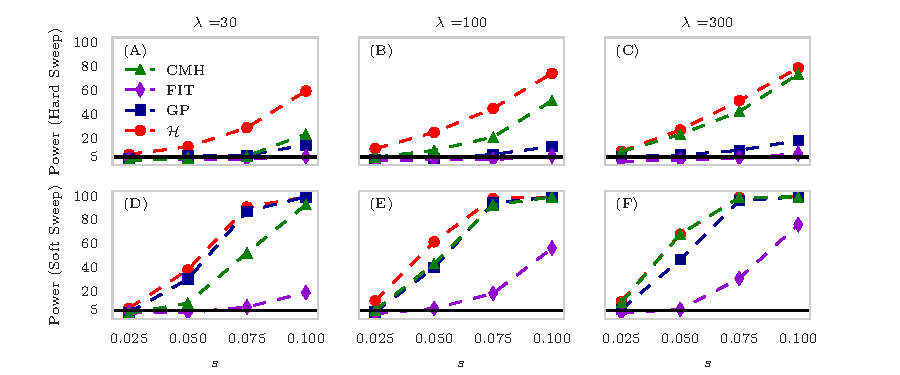
\includegraphics[trim=.2in 0 .2in 0 , clip,width=\textwidth]{figures/power.pdf}
	\caption{Predictive performance of different method is evaluated on 1000 
		simulations for different values of selection strength $s$ and initial 
		carrier frequency $\nu_0$.} \label{fig:power}
\end{figure}
\begin{figure}[H]
	\centering
	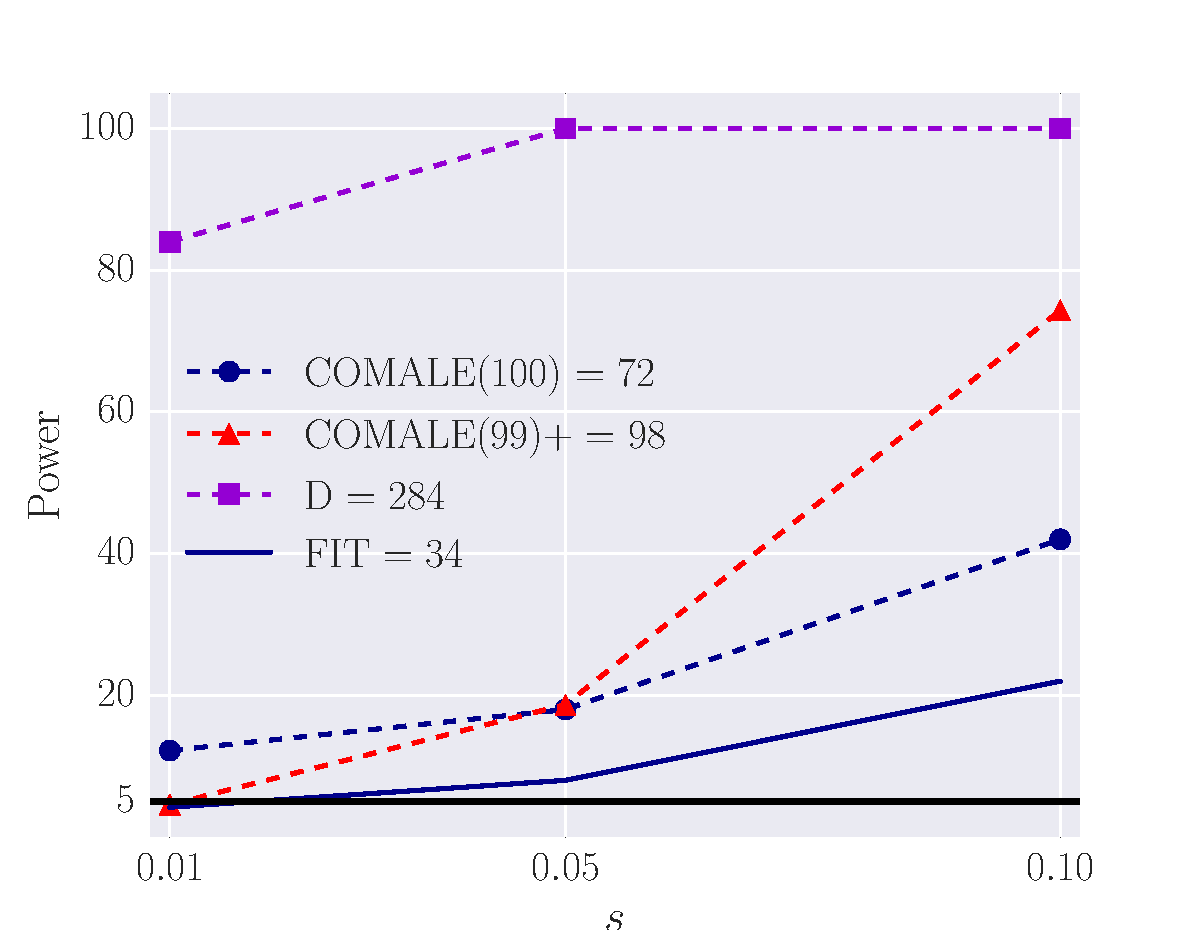
\includegraphics[trim=.2in 0 .2in 0 , clip,width=\textwidth]{figures/powerSFS.pdf}
	\caption{Predictive performance of different method is evaluated on 400 
		simulations for different values of selection strength $s$ and initial 
		carrier frequency $\nu_0$.} \label{fig:powerSFS}
\end{figure}

\begin{figure}[H]
	\centering
	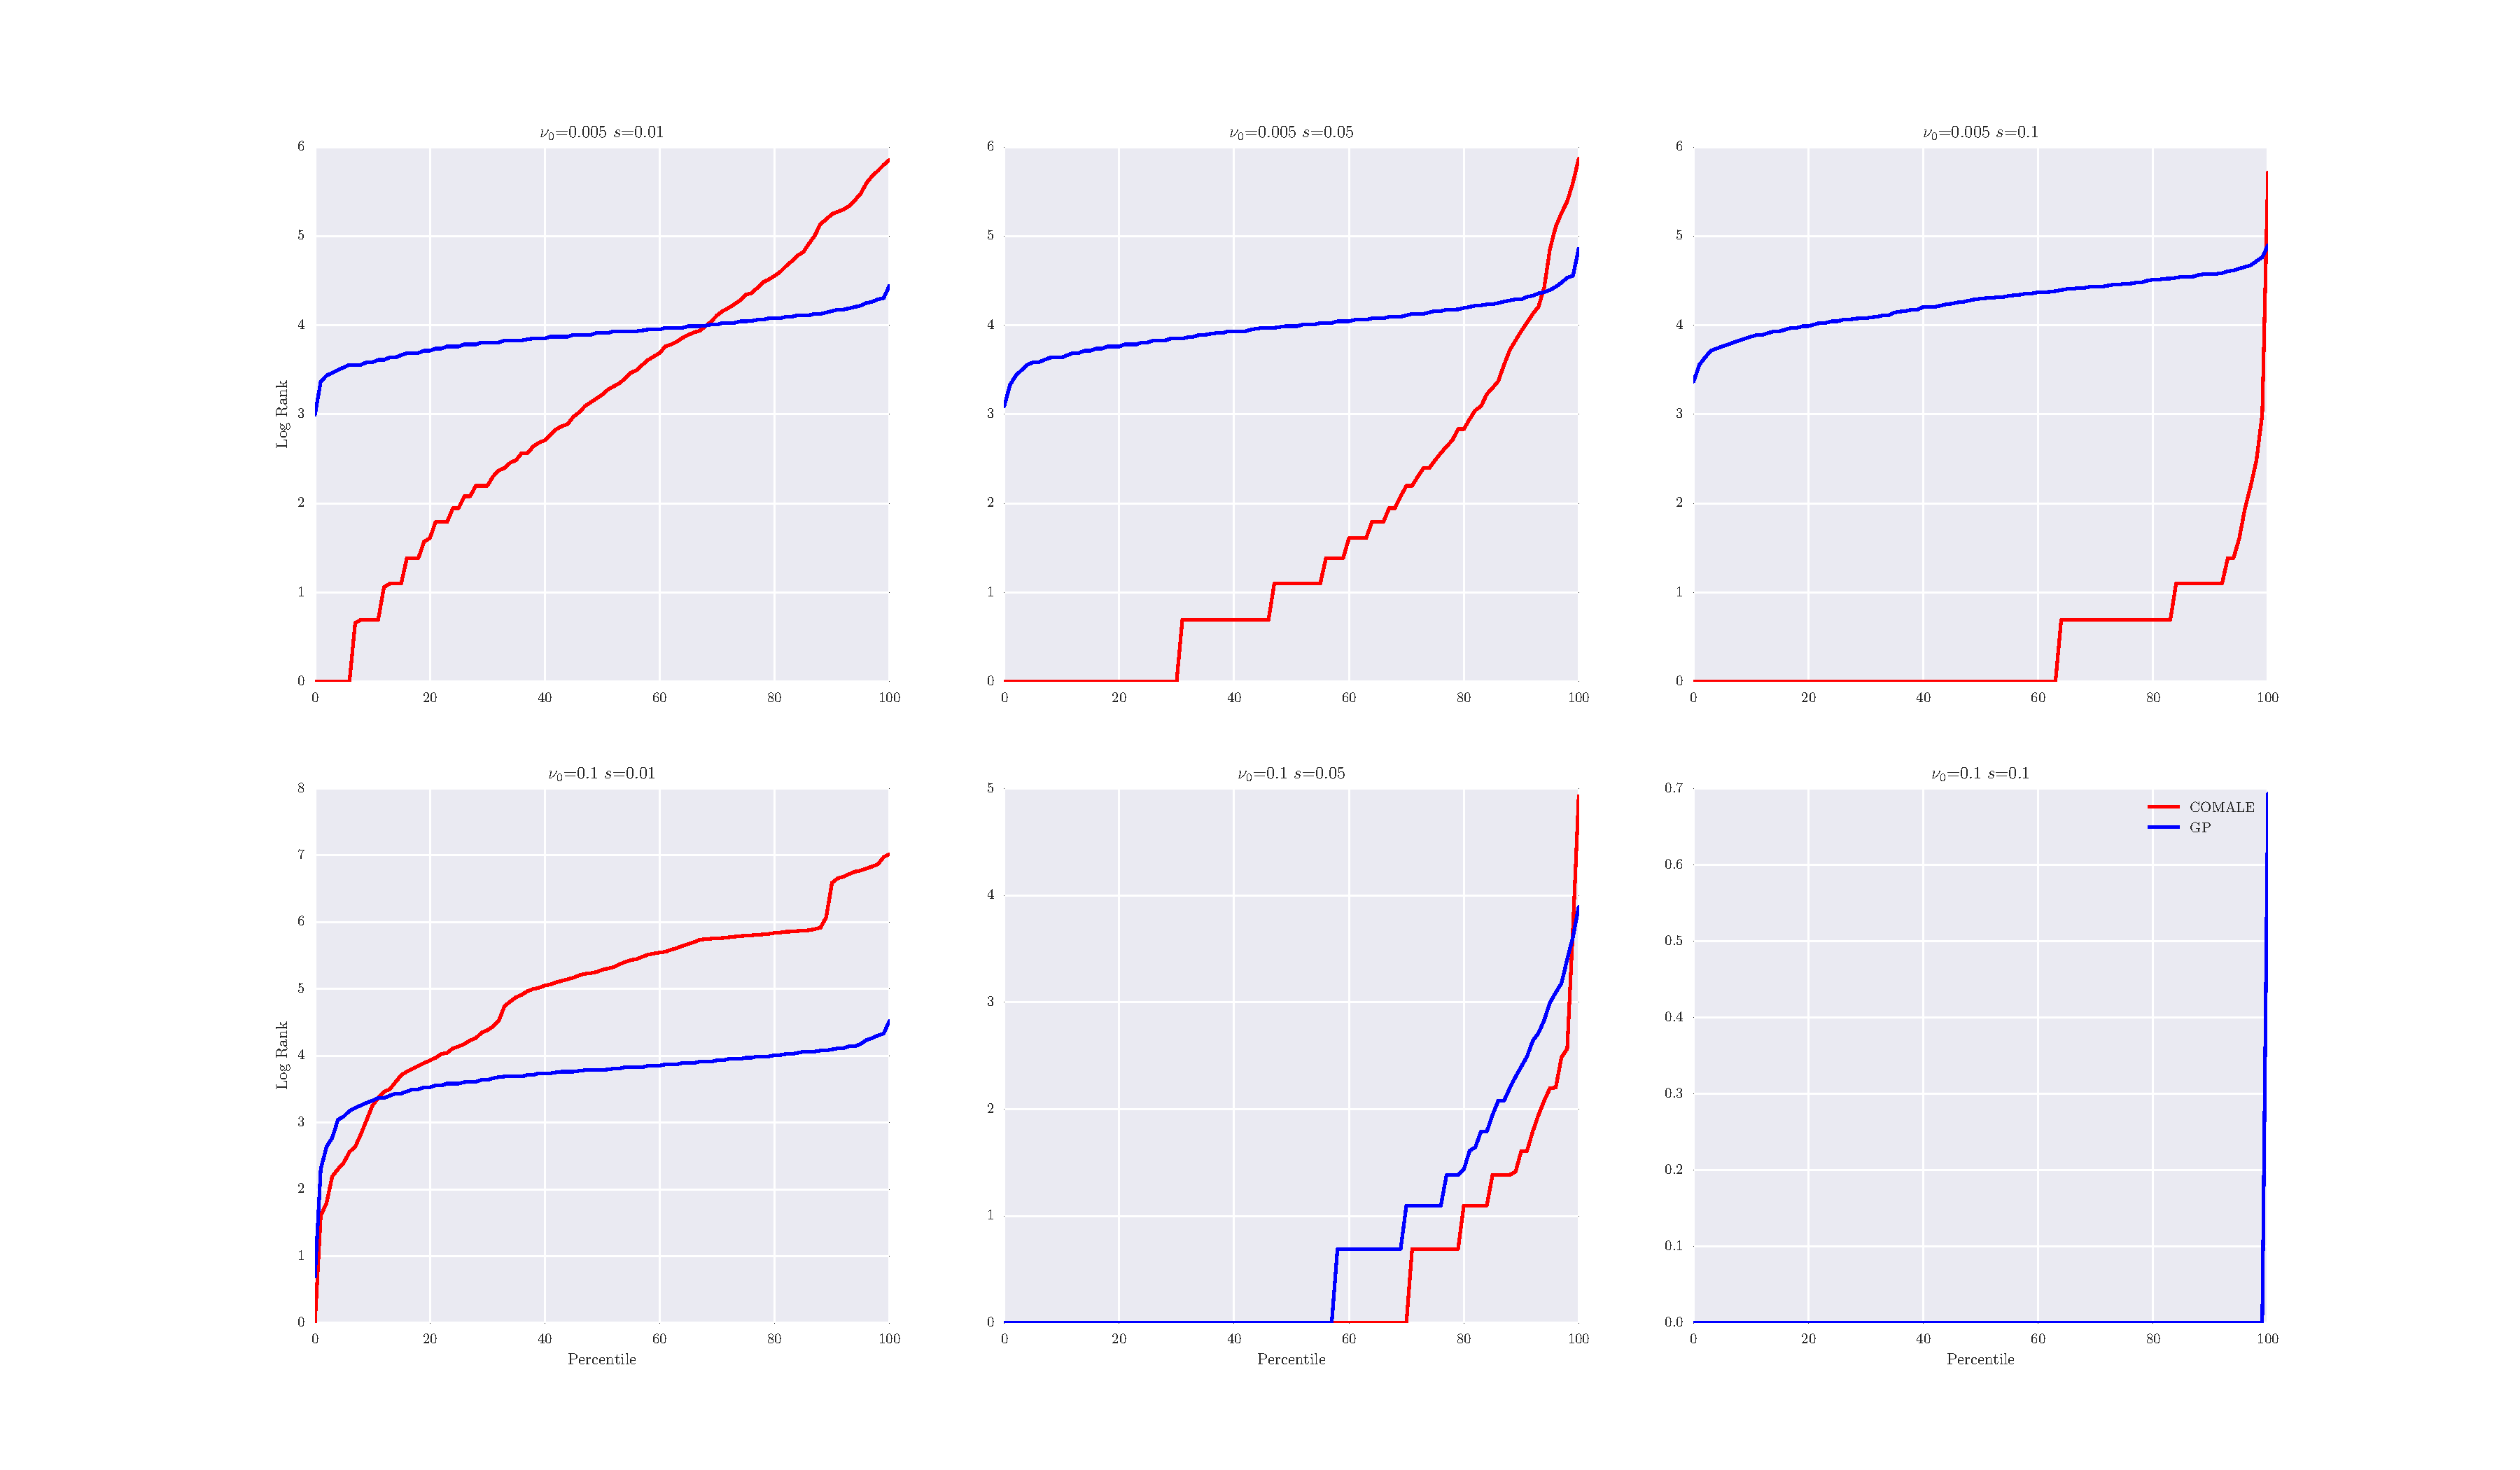
\includegraphics[trim=.2in 0 .2in 0, 
	clip,width=\textwidth]{figures/rank.pdf}
	\caption{CDF of the rank of the adaptive allele in 100
          simulations. \VB{Please put rank (not log rank) in X-axis,,
            and CDF on the Y-axis. In other words if the rank is 10,
            the y-axis should give the fraction of simulations in
            which the rank was 10 or better. Also, font size is way
            too small. Please make it larger.}}
	\label{fig:rank}
\end{figure}


\begin{figure}[H]
	\centering
	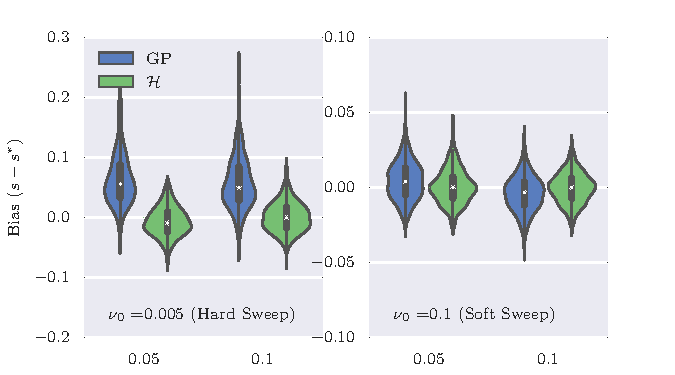
\includegraphics[trim=.2in 0 .2in 0 , clip,width=\textwidth]{figures/bias.pdf}
	\caption{\VB{Font size, and please write a caption}.} \label{fig:bias}
\end{figure}


\begin{figure}[H]
	\centering
	\includegraphics[width=\textwidth]{figures/{manhattanSNP.png}}\\	
	\includegraphics[width=\textwidth]{figures/{manhattanSNP.Genes}.pdf}
		\caption{Manhattan plots shows the distribution of candidate (top 2000) 
		SNPs and the associated (1961) genes are denoted with blue line in the bottom plot.} 
	\label{fig:realsnp}
\end{figure}

\begin{figure}[H]
	\centering
		\includegraphics[width=\textwidth]{figures/{manhattanWindow.pdf}}\\	
			\includegraphics[width=\textwidth]{figures/{manhattanWindow.Genes}.pdf}
	\caption{Manhattan plots shows the distribution of candidate regions using \comale statistic which give rise to (421) genes are denoted with blue line in the bottom plot.} 
	\label{fig:realcomale}
\end{figure}


\begin{figure}[H]
	\centering
	\includegraphics[width=\textwidth]{figures/{runTime.pdf}}
	\caption{Running time of GP and \comale.} 
	\label{fig:runTime}
\end{figure}

%\section{Introduction}

Genetic adaptation is \emph{the} central evolutionary process and is
at the core of some of the greatest challenges facing humanity. HIV
would likely cause nothing more than harmless fever without the
ability of the virus to adapt and eventually destroy the immune
system. Cancer would be much more straightforward to treat if not for
tumor's ability to adapt to anti-cancer drugs. Malaria could be
treated with cheap drugs such as quinine instead of being one of the
world's worst killers. Crop pests would be manageable with small doses
of safe insecticides instead of requiring applications of ever
increasing amounts of a diverse array of powerful chemicals. In both
disease and agriculture, we find ourselves in an arms race due to the
ability of organisms to adapt.

Adaptation leaves a variety of detectable signatures in
genomes~\cite{Akey09, Kreitman00, MesserAndPetrov13, Nielsen05,
  SabetiEtAl06}. The rapid expansion of adaptive alleles in
populations leads to both an excess of functional changes between
species and distortions in polymorphism patterns known as selective
sweeps~\cite{Nielsen05}. The signatures of selective sweeps, which
include reduction of levels of polymorphism and the presence of too
many rare alleles~\cite{Nielsen05, Przeworski02}, have been the basis
for assessing genomic patterns in many genome scans for
adaptation. Classical tests such as the well-known Tajima's \emph{D}
statistic~\cite{Tajima89} that rely on the \emph{site-frequency
  spectrum}---a list of counts of the numbers of genomic sites in a
region with each of the different possible allele frequencies---have
been among the first steps in genomic detection of selection, but they
have largely been chosen in a non-systematic manner to identify quite
specific rather than general signatures of selection, and they have
often faced the problem of confounding of positive selection with
demographic processes~\cite{PtakAndPrzeworski02, RamosOnsinsAndRojas}.
Part of the challenge is that studies on natural populations are
conducted on a extant populations, a single window in a complex,
uncontrolled process.

Experimental evolution (including evolve and re-sequence paradigms)
have become increasingly popular as a complementary tool to understand
the forces of selection, allowing for controlled environments,
specific selection constraints. Examples of experimental evolution
studies abound in sexual populations, particularly in fruitfly. Burke
et al.~\cite{Burke2010} evolved flies for over $600$ generations under
selection for accelerated development, and noted that evolution for
sexual populations is very different from those of asexual populations
(e.g., Lenski~\cite{}): the effects of clonal interference is slower
due to recombination that allows for the incorporation of multiple
beneficial alleles, but there are fewer, unconditionally advantageous
alleles that arise at the onset of selection. Rose and
Colleagues~\cite{Rose} created $200$ experimentally evolved
populations selected for different traits, starting with $10$ initial
populations. Zhou et al. evolved flies to adapt to low oxygen
environment (hypoxia) for over $300$ generations, and identified many
genes involved in hypoxia tolerance~\cite{}.  Instead, they observed
incomplete fixation (`soft-sweeps') due in part to standing variation,
changing selection coefficients, and small fitness effects.

Much like in natural populations, many of these studies also
sequenced/genotyped only the latest population. However, the emergence
of NGS and related technologies has made it feasible to sequence the
evolving population at multiple time points in its evolution. At the
same time, for small organisms where a single animal does not provide
enough DNA, it is more effective to pool together individuals in the
population at a particular time point, in a single sequencing
experiment. Thus, instead of individual genotypes, we obtain
frequencies of the derived allele at all loci at different time
points. Methods for analyzing such time series pooled sequence data
are only just being developed.

In this paper we aim to use the tools and machinery that has been
developed for RNNs, to model times-series biological data. In
particular, we consider the population genetics problem of finding
loci (locus) under selection given observation of allele frequency of
a population in different generations of a Wright-Fisher model. This
problem has been previously treated by using Gaussian Processes
\cite{EnadR-GP}, spectral methods \cite{EandR-spectral}




%\section{Methods}
In this section we formally present describe RNN model and a Naive method which takes $\Oc(1)$ computations as baseline performance.

\subsection{Notation}
In this paper, we denote Tensor with bold-faced capital letter, matrices with capital letter, vectors with bold-faced small letter, and scalars with small letters. Let $\bfX \in [0,1]^{R \times T \times L}$  be the Tensor of containing allele frequencies of the population where $R,L,T$ are number of experimental replicates, samples in time, segregating sites, respectively. Also, in our simplified notation $X_r=[\bfx_1 ,\cdots, \bfx_L]\in  [0,1]^ {T \times L}$  data matrix for replicate $r$,  $\bfx_l =[x_1,\cdots,x_T]$ is the observation at locus $i$ for a given replicate, and $x_t\in [0,1]$ is the allele frequency at time $t$ for a given replicate and locus. It should be noted that $T=|\Tc|$ where $\Tc=\{\tau_1,\tau_2,\cdot, \tau_T \}$ is the set of times (generations) of samples which pool sequencing data is collected. For examples $\Tc=\{2,18,25\}$ denotes that the dataset contains allele frequency of the population at 2nd, 18th and 25th generations.



\subsection{Regularized Nonlinear Least Squares}
For simplicity, in this paper we consider bi-allelic single-locus Wright-Fisher (WF) model with no mutations \cite{book-mathpopgen} which assumes  discrete generation, random mating etc. Under finite population size\footnote{In infinite population size we have $x_{t+1} = f(x_t;s,h)$.} assumption allele frequency at each generation is a random variable
\beq\label{eq:trans0}
x_{t+1} = f(x_t;s,h)  + \epsilon_t
\eeq
where $h$ is the overdominance, $\epsilon_t$ is random noise due to genetic drift at generation $t$ and $f: [0,1] \mapsto [0,1]$ is the transition function:
\beq
f(x)=\frac{(1+s)x^2 + (1+hs)x(1-x)}{(1+s)x^2 + 2(1+hs)x(1-x) + x(1-x)}=x+\frac{s(h+(1-2h)x)x(1-x)}{1+sx(2h+(1-2h)x))}
\eeq
Since the transition function depend on both $s$ and $h$, we can estimate both of them at the same time by solving a 2-dimensional optimization problem. However, for the sake of simplicity of notation we aim to only estimate $s$ and set $h=0.5$ 
\beq
f(x)=x+\frac{sx(1-x)}{2+2sx}
\eeq
Given $x_t$, we can consider \ref{eq:trans0} as a nonlinear function of $s$ and finding $s$ can be formulated as a classical a 1-dimensional non-linear least-squares problem \cite{•}
\beq \label{eq:nlls0}
s^*=\underset{s}{\arg \min} \| x_{t+1} -f(x_t;s,h)\|^2
\eeq
which can be solved by iterative optimization algorithms. 
However, \eqref{eq:nlls0} does not account for dependence of $x_t,x_{t-1}, \cdots$ to $s$. To incorporate this dependence, we introduce the notation
\beq
y_t(s)= \underbrace{f(\cdots f(}_tx_0;s))
\eeq
and we can find $s$ by solving
\beq
s^*=\underset{s}{\arg \min} \sum_{t=1}^T \| y_{\tau_t}(s)- x_{t} \|^2
\eeq
On the other hand, using ordinary differential equations (ODE), \eqref{eq:trans0} can be written as \cite{multilocus-hitchhike}:

\beq
y_t(s)=\frac{x_0}{x_0 +(1-x_0)e^{-s\tau_t/2}}= \frac{1}{1+ce^{-s\tau_t/2}} = \sigma(-s\tau_t/2)
\eeq
where $c=(1-x_0)/x_0$ is constant and $\sigma(.)$ is modified sigmoid function (due to presence of $c$). Therefore, we have
\beq
s^*=\underset{s}{\arg \min} \sum_{t=1}^T \frac{1}{2} \| \sigma(s\tau_t/2)- x_{t} \|^2 + \frac{\lambda }{2}s^2
\eeq
which is a standard 1-d nonlinear regularized nonlinear least squares (RNLLS) optimization problem. To solve it we need to use iterative optimization algorithms which require computing gradient\footnote{$\sigma'(s)=\sigma(s)(1-\sigma(s))$} w.r.t. $s$
\beq
g= \sum_{t=1}^T \frac{\tau_t}{2} ( \sigma(s\tau_t/2)- x_{t} ) \sigma(s\tau_t/2) (1-\sigma(s\tau_t/2)) + \lambda s
\eeq
By taking into account of all replicates, the gradient descent update is
\beq
s\leftarrow s - \eta \sum_{r=1}^R g_i
\eeq
where $\eta$ is learning rate. Also, since this problem is not convex, we use Nestrov's Accelerated Gradient (NAG) descent algorithm which which has shown to be successful on many nonconvex problems. Also it should be noted that each iteration of the optimization takes $\Oc(TR)$ computation which make the algorithm tractable.

\subsection{Gaussian Process}
The Gaussian Process optimizes
\beq
\underset{\theta}{ \arg \max} \ \ \Lc(\bfX | \theta)
\eeq
where $\Lc$ is Gaussian distribution log-likelihood, i.e. negative weighted least-squares loss. Mean and covariance functions of the GP at any $t,l$ are functionally dependent to parameter of interest $\theta$, and computed using transition function of the WF process \cite{EandR-GP}.

\subsection{Naive Method}
To have a baseline performance,  in this subsection we consider a scenario with infinite population size, i.e., 
\beq
x_t(s)=\frac{x_0}{x_0 +(1-x_0)e^{-s\tau_t/2}}
\eeq
Since $s$ assumed to be constant, we can solve for $s$
\beq
s_t=\frac{2}{\tau_t} \log \left( \frac{x_t (1-x_0)}{x_0 (1-x_t)} \right)
\eeq
and finally to reduce the variance we can average all the naive estimates:
\beq
s_{Naive}=\sum_{t=1}^T\frac{2}{\tau_t} \log \left( \frac{x_t (1-x_0)}{x_0 (1-x_t)} \right)
\eeq

%\section{Methods (Arya)}
\beq
  \frac{d\nu_t(s)}{dt} &=\frac{s}{2}\nu_t(s)(1-\nu_t(s))\frac{1}{1+s\nu_t(s)} \\
  \frac{st}{2}-c&=\log\left(\frac{\nu_0}{(1-\nu_0)^{1+s}}\right)
  
\eeq
\section{Experiments}
In this part we compare MLE with GP and Naive method. 
\subsection{Data}
\subsubsection{Simulations}
For each experiment a diploid population is created and evolved as follows. 
\paragraph{I. Creating initial founder lines}
First using msms prgram, we created a population for $F$ founding haplotypes with parameters \texttt{\$./msms <F> 1 -t <4μLNe> -r <4Ne(L − 1)r> <L>} where $F=200$ is number of founder lines, 
$L=10^5$, $\theta=4\mu LNe=17$ and $\rho=4Ne(L-1)r=4$.  (assuming $Ne=1000$, $r=10^{-8}$ and $\mu=4.25\times 10^{-8}$).  
\paragraph{II. Creating initial diploid population} 
To mimic the real E\&R experiment for diploid organisms, first initial haplotypes cloned to create $F$ diploid homozygotes. Then each diploid is cloned $N/F$ times to yield $N$ diploid homozygote organisms.
\paragraph{III. Forward Simulation}
Given initial diploid population, position of the site under selection, selection strength $s$, number of replicates $R=3$, recombination rate $r=10^{-8}$ and sampling times $\Tc=\{10,20,30,40,50\}$ simuPop is used to perform forward simulation and compute allele frequencies for all of the $R$.

\subsubsection{Real}

\subsection{Likelihood Ratio Test}
Using the MLE (and other) estimates of $s$ it is desirable to perform a secondary task such as \emph{testing for selection} or \emph{locating the site under selection}. Likelihood ratio test (LRT) statistics for time series \cite{feder2014} have shown to be predictors for differentiating neutral and natural selection evolution cases. For a single locus model, the likelihood ratio test statistics $\Lambda(s*)$ is defined
\beq \label{eq:lrt}
\Lambda(s^*) = \log \left(\frac{\Lc(\bfX|s=s*)}{\Lc(\bfX|s=0)}\right)
\eeq
where $s^*$ is the optimal solution for the maximum-likelihood procedure. For the Gaussian process and Gaussian model the likelihood $\Lc_{GP}$ and $\Lc_G$ are well defined and \eqref{eq:lrt} can be easily evaluated. The likelihood of the Naive method for estimating based on $x_t$ is 
\beq
\Lc_N(s|x_t,x_0)=x_t-\sigma(st/2 -c)
\eeq

In addition to LRT, the value of $s^*$ itself can be regarded as a signal for detecting selection. In other words, modifying the LRT to
\beq
\Theta=s^*\Lambda(s^*)
\eeq
will take into account of two different objectives, 1)model discrepancy from neutral model 2)strength of selection under non-neutral model. In the  results we show that the modified-LRT makes more accurate predictions.

\subsection{Results}
In this part we compare the computational and predictive performance of the proposed method in detecting selection, locating selection in the genome, and estimating strength of selection with Gaussian process and the outlined naive method.

\subsubsection{Detecting Selection}
Detecting selection in the whole genome is a non-trivial task in real world and can be regarded as a application for the proposed algorithm. To provide a fair and unbiased comparison, we computed the test statistic for 1000 simulations and computed Receiver Operative Characteristic curve and Area Under Curve (AUC) for each method.



\begin{figure}[H]
  \centering
    \includegraphics[width=\textwidth]{{roc0.01A0.01}.png}
  \caption{Rank}
  \label{fig:Fig3a}
\end{figure}

\begin{figure}[H]
  \centering
    \includegraphics[width=\textwidth]{{roc0.02A0.01}.png}
  \caption{Rank}
  \label{fig:Fig3b}
\end{figure}

\begin{figure}[H]
  \centering
    \includegraphics[width=\textwidth]{{roc0.05A0.01}.png}
  \caption{Rank}
  \label{fig:Fig3c}
\end{figure}

\begin{figure}[H]
  \centering
    \includegraphics[width=\textwidth]{{roc0.1A0.1}.png}
  \caption{Rank}
  \label{fig:Fig3d}
\end{figure}

\begin{table}
\centering
\begin{tabular}{ l |c c c c }
$s$& 0.01 &0.02 & 0.05 & 0.1 \\
\hline
  Gaussian Model & 2 & 3& 2 & 3 \\
Gaussian Process & 5 & 6 & 2 & 3\\
  Naive & 8 & 9 & 2 & 3\\
\end{tabular}
\caption{AUC of all method evaluated for 1000 simulations and different values of $s$.}
\end{table}


\subsubsection{Finding Site Under Selection}
\paragraph{Distance}
\begin{figure}[H]
  \centering
    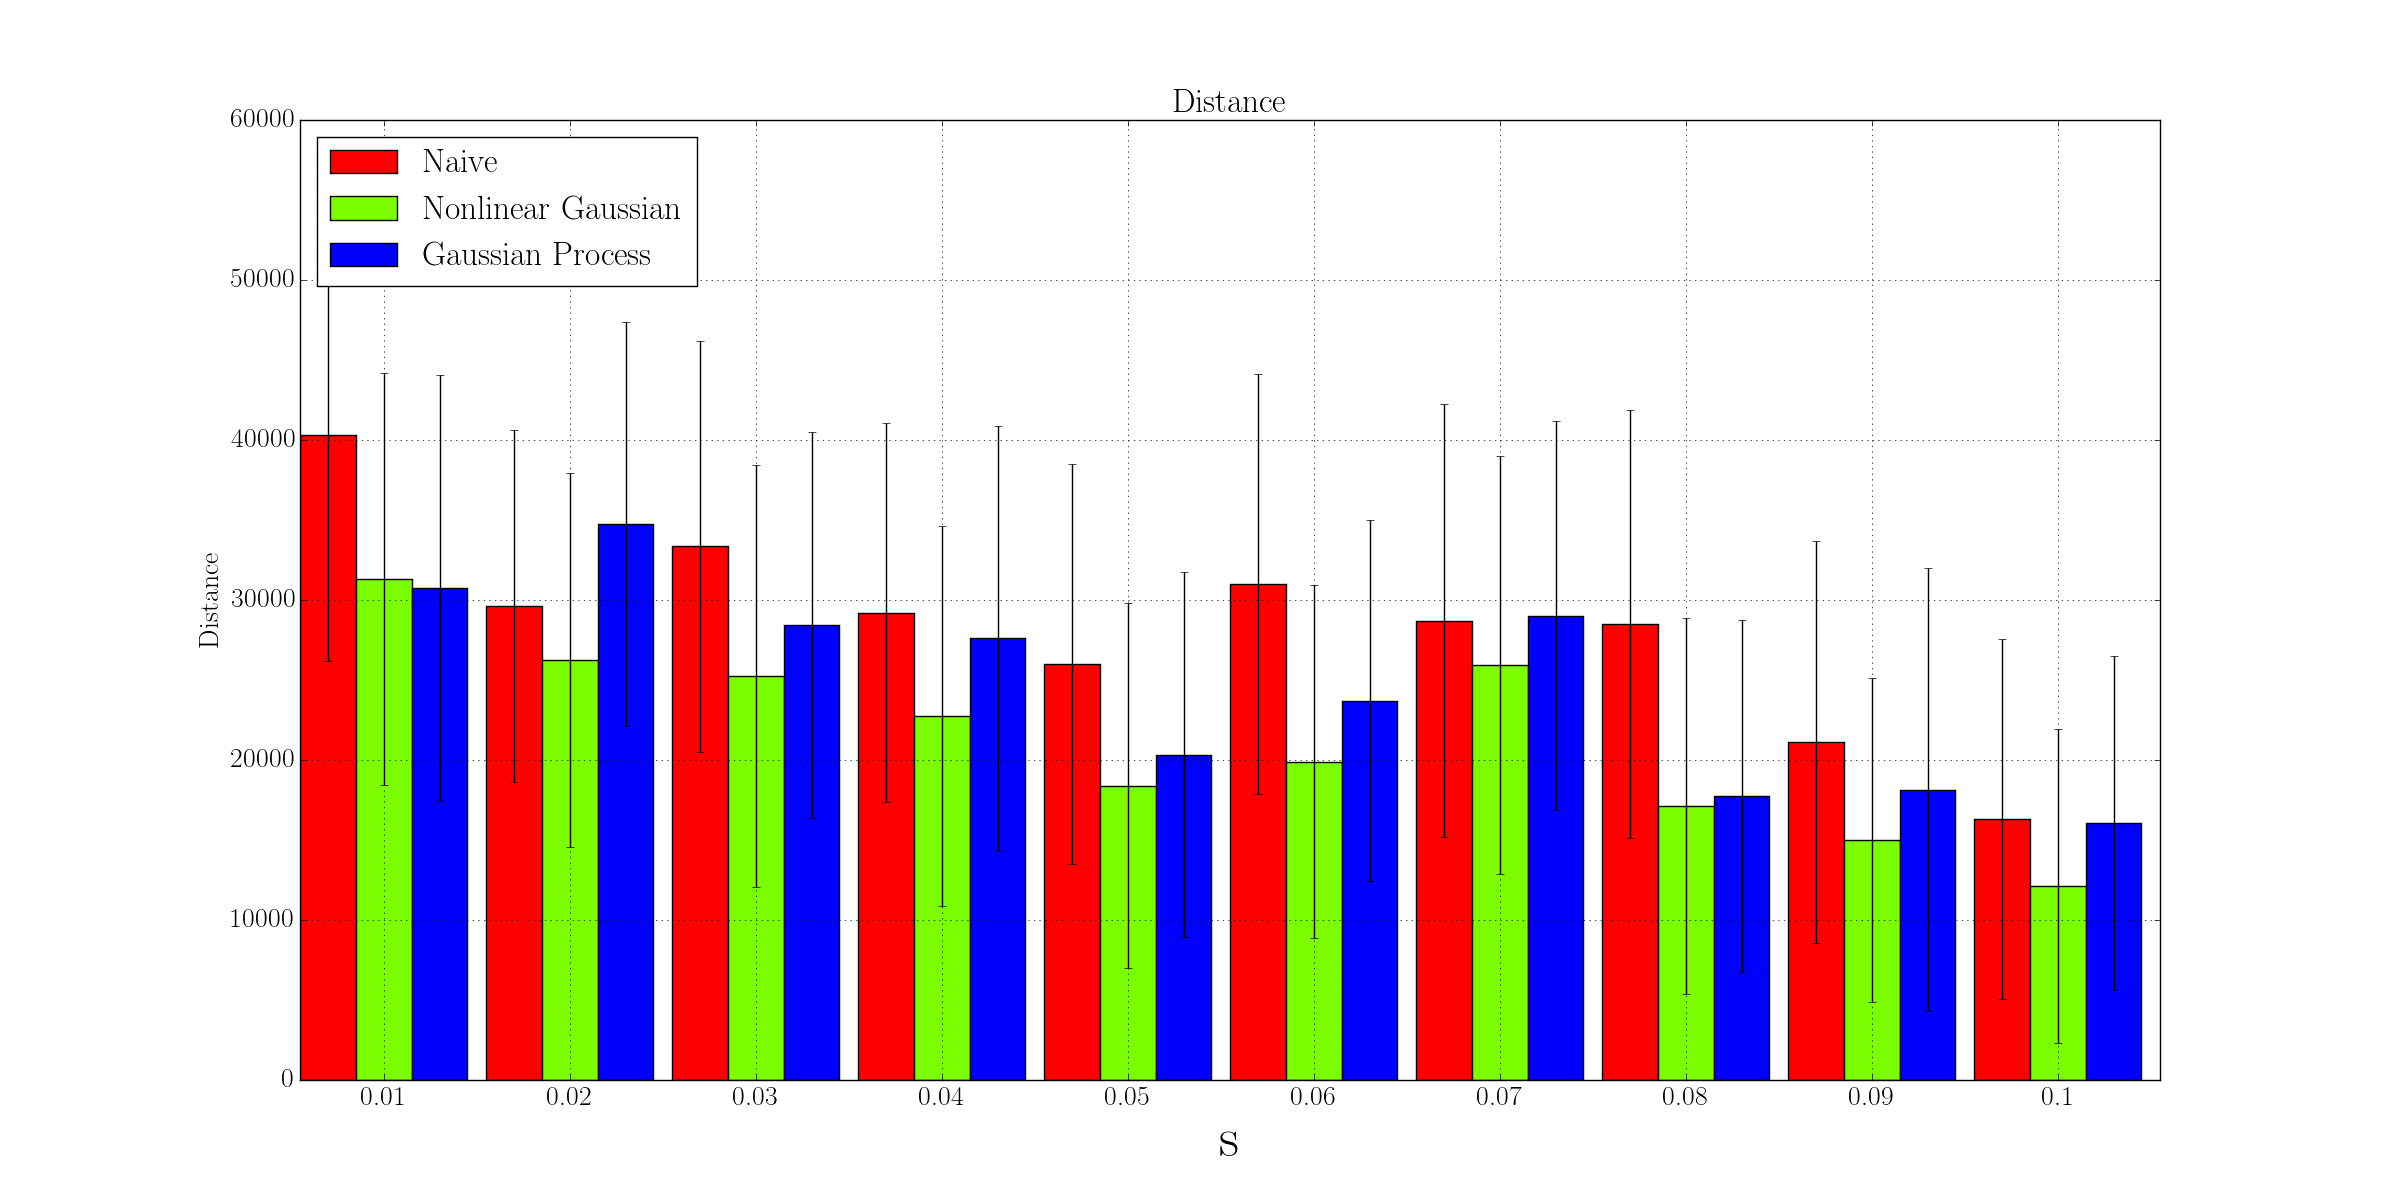
\includegraphics[width=\textwidth]{dist}
  \caption{Average distance to predicted site to the true site that is under selection.}
  \label{fig:Fig1}
\end{figure}

\paragraph{Rank}
\begin{figure}[H]
  \centering
    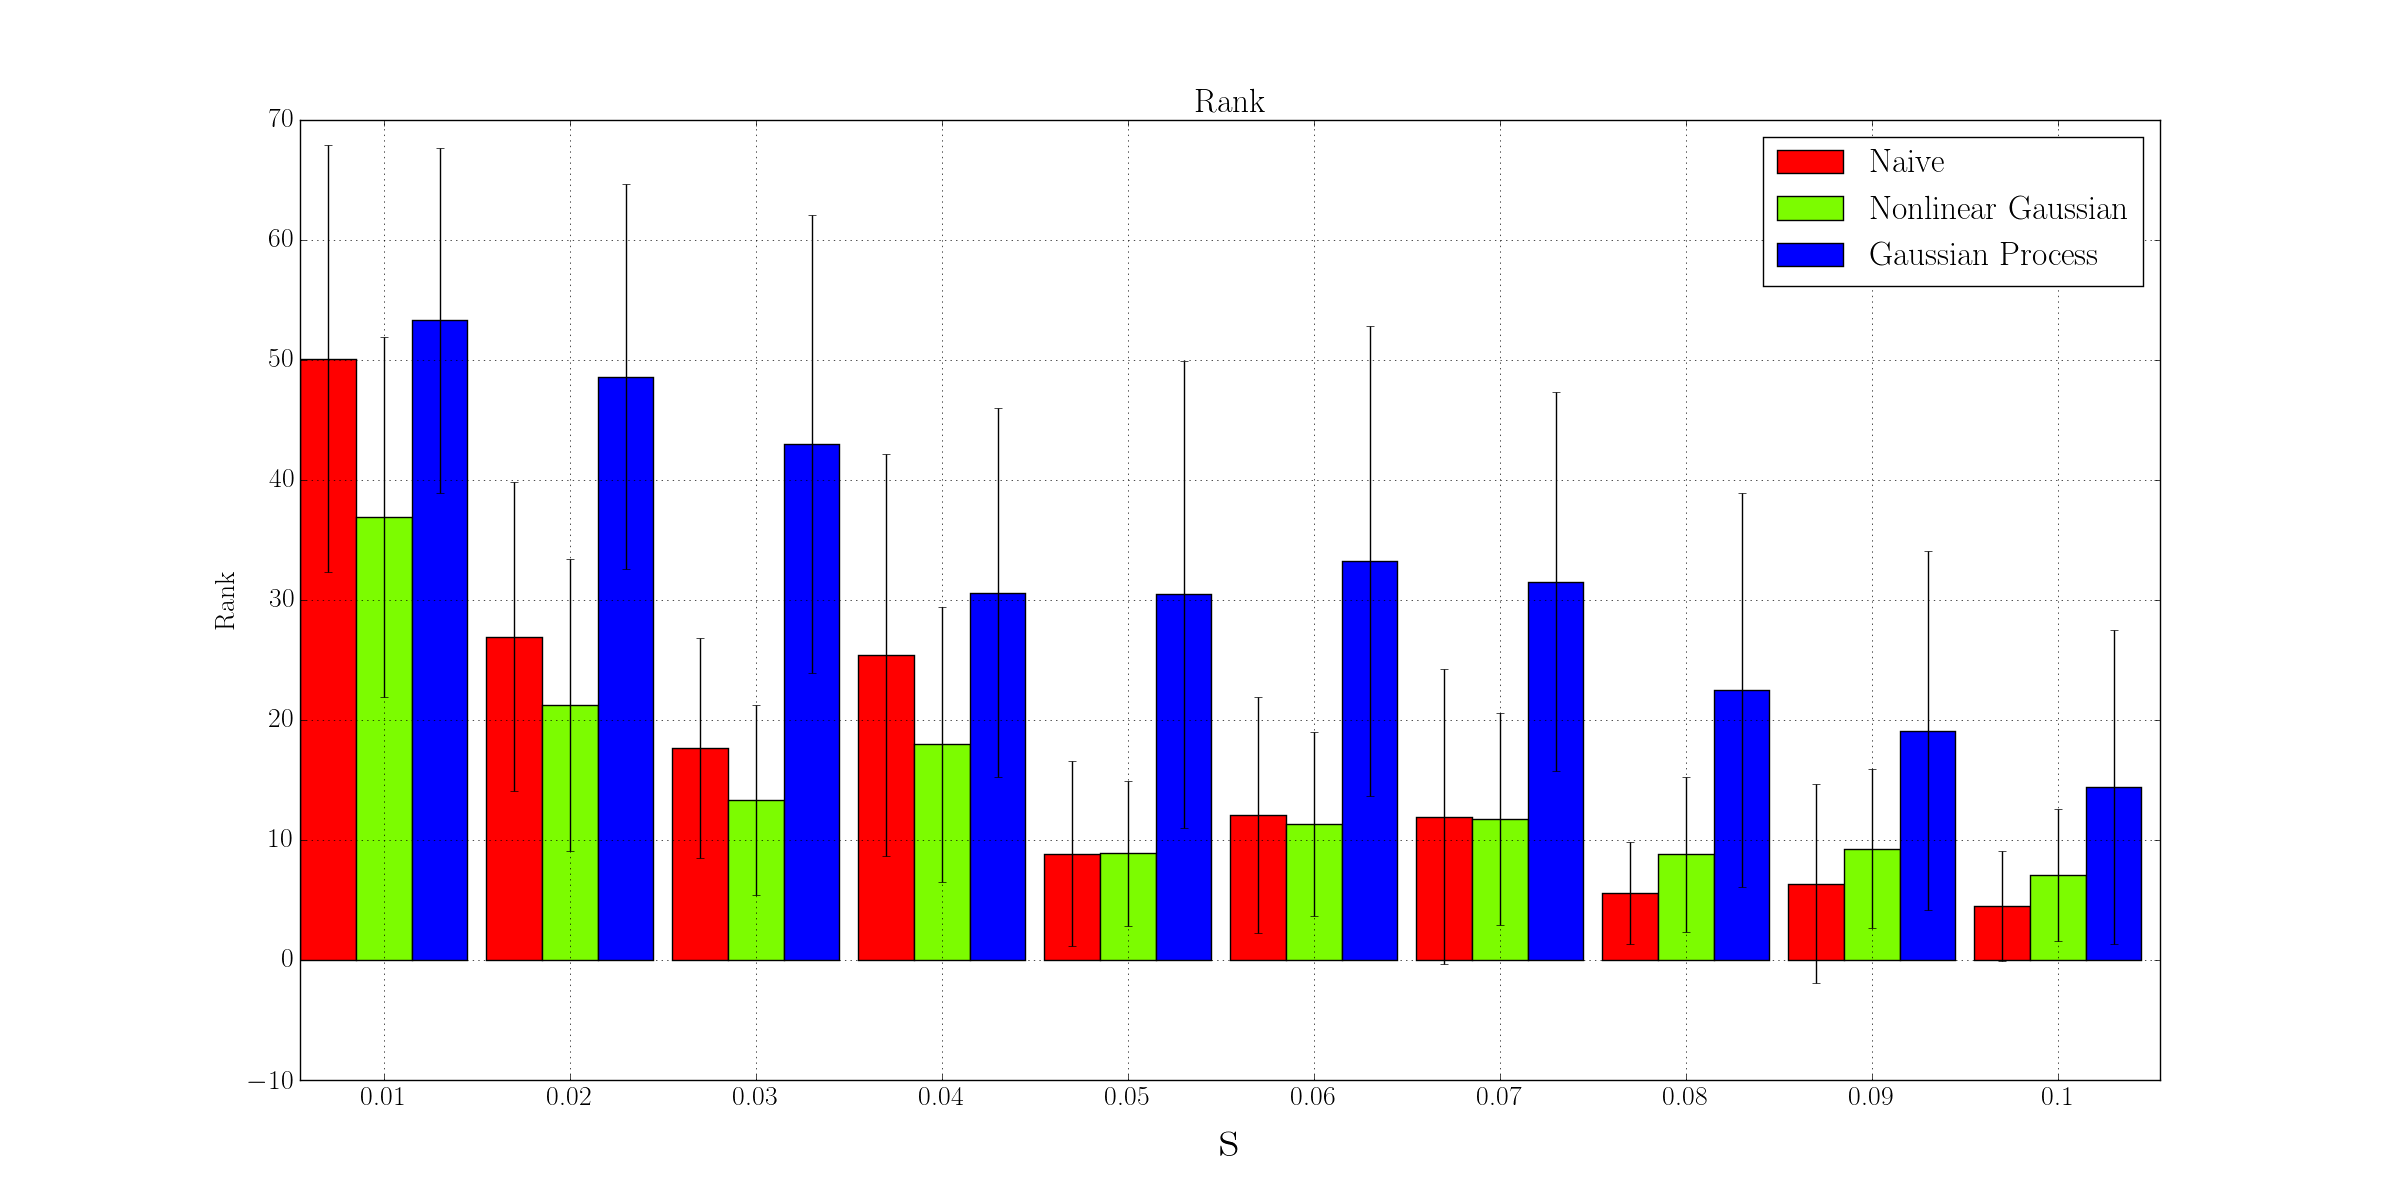
\includegraphics[width=\textwidth]{rank}
  \caption{Rank}
  \label{fig:Fig3}
\end{figure}

\paragraph{Mean Reciprocal Rank(MRR)}
\begin{figure}[H]
  \centering
    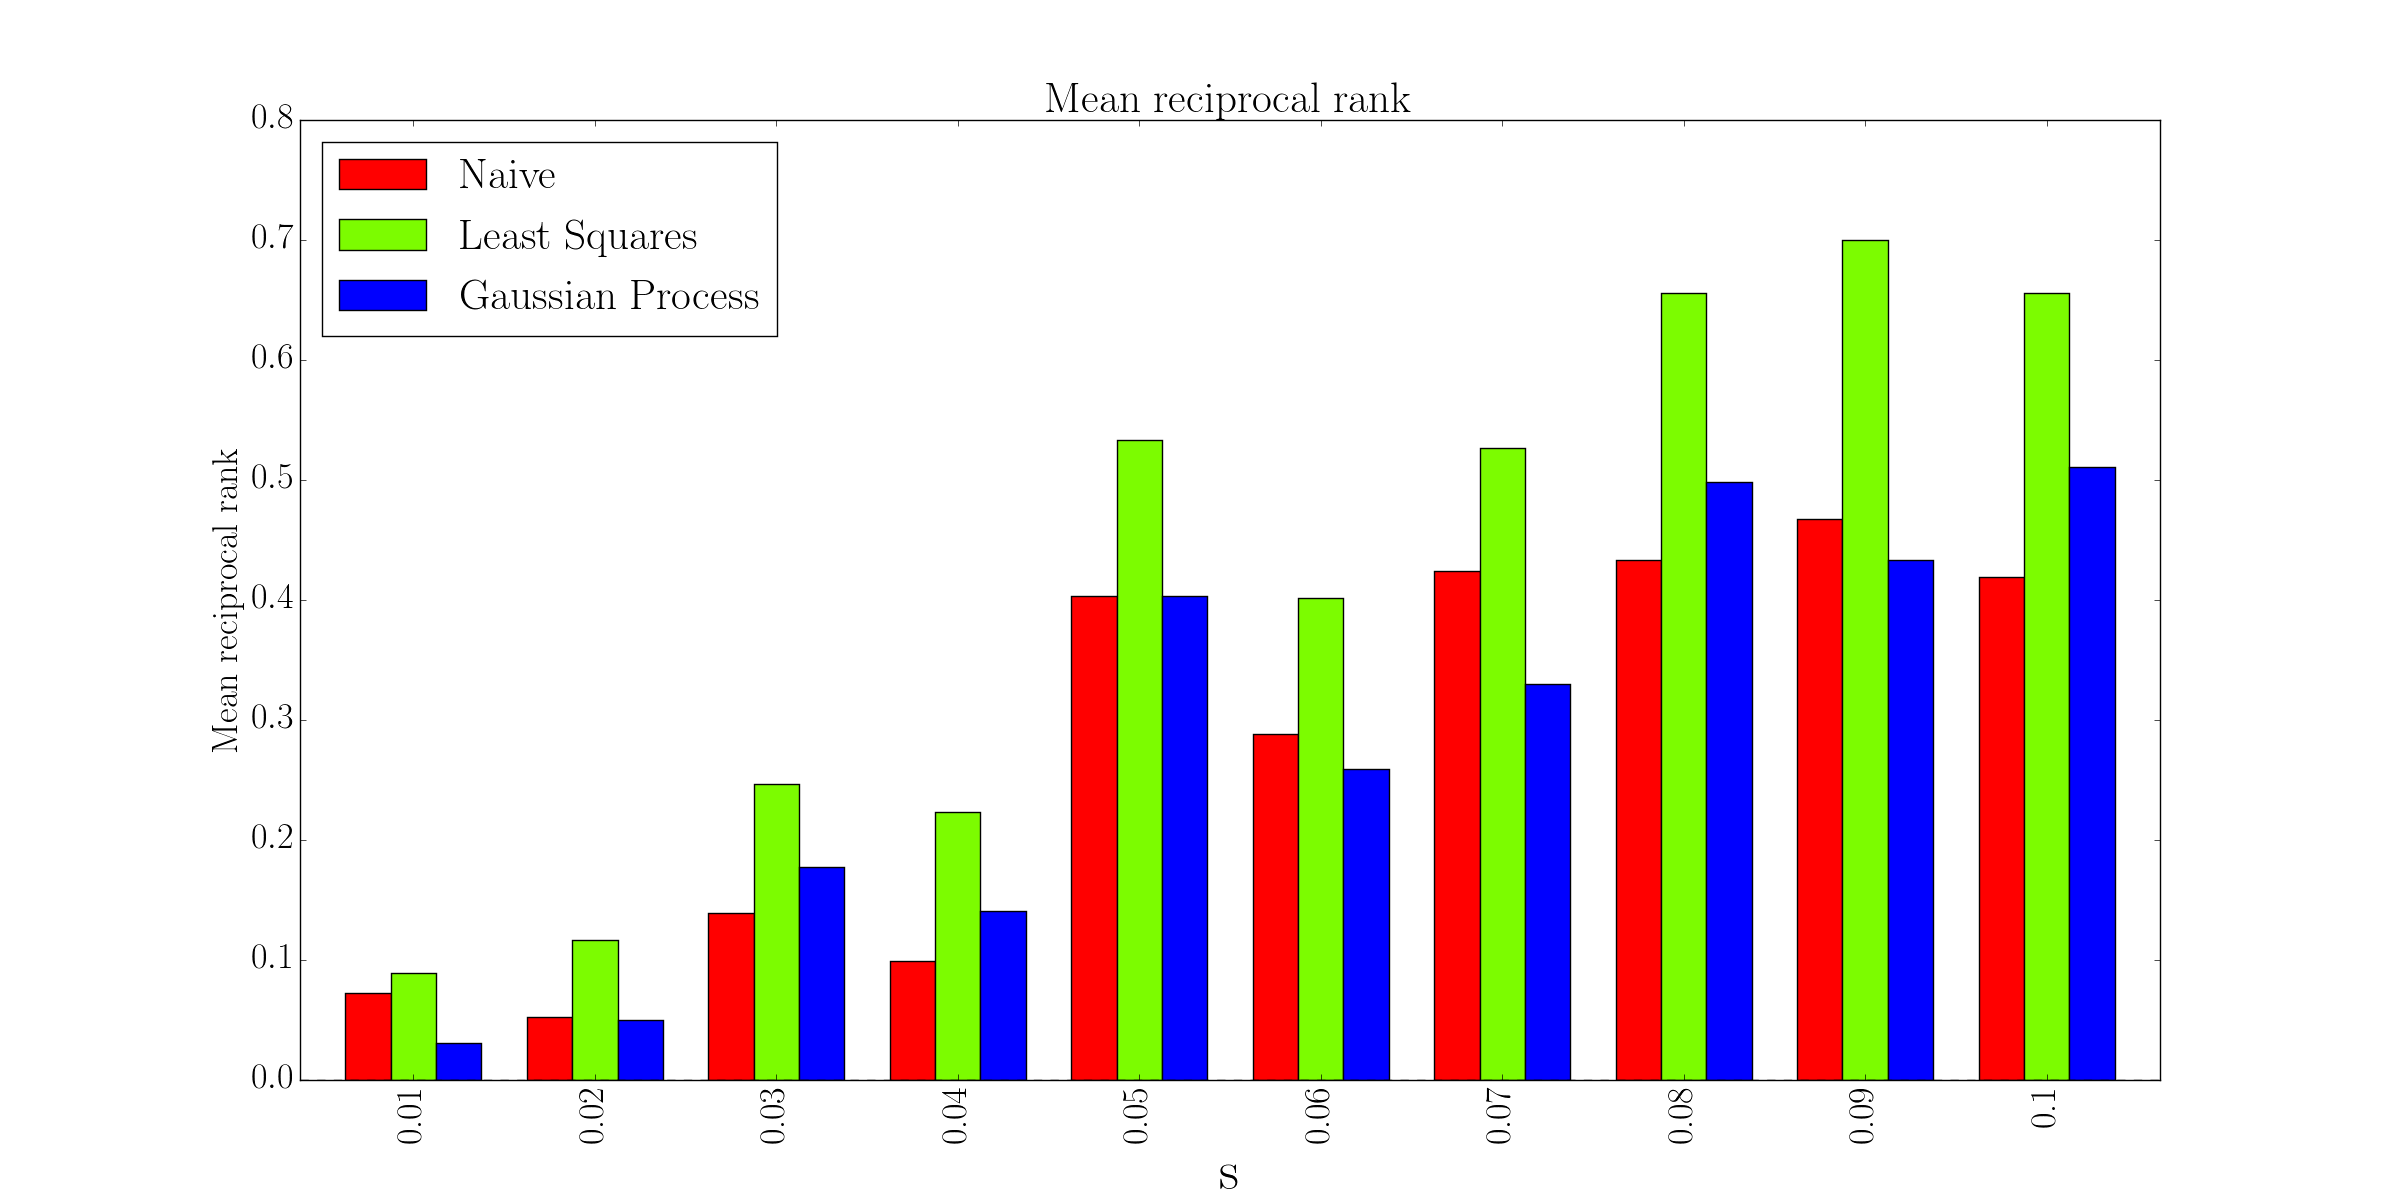
\includegraphics[width=\textwidth]{mrr}
  \caption{Mean Reciprocal}
  \label{fig:Fig2}
\end{figure}


\paragraph{Mean Average Precision (MAP)}
\begin{figure}[hh]
  \centering
    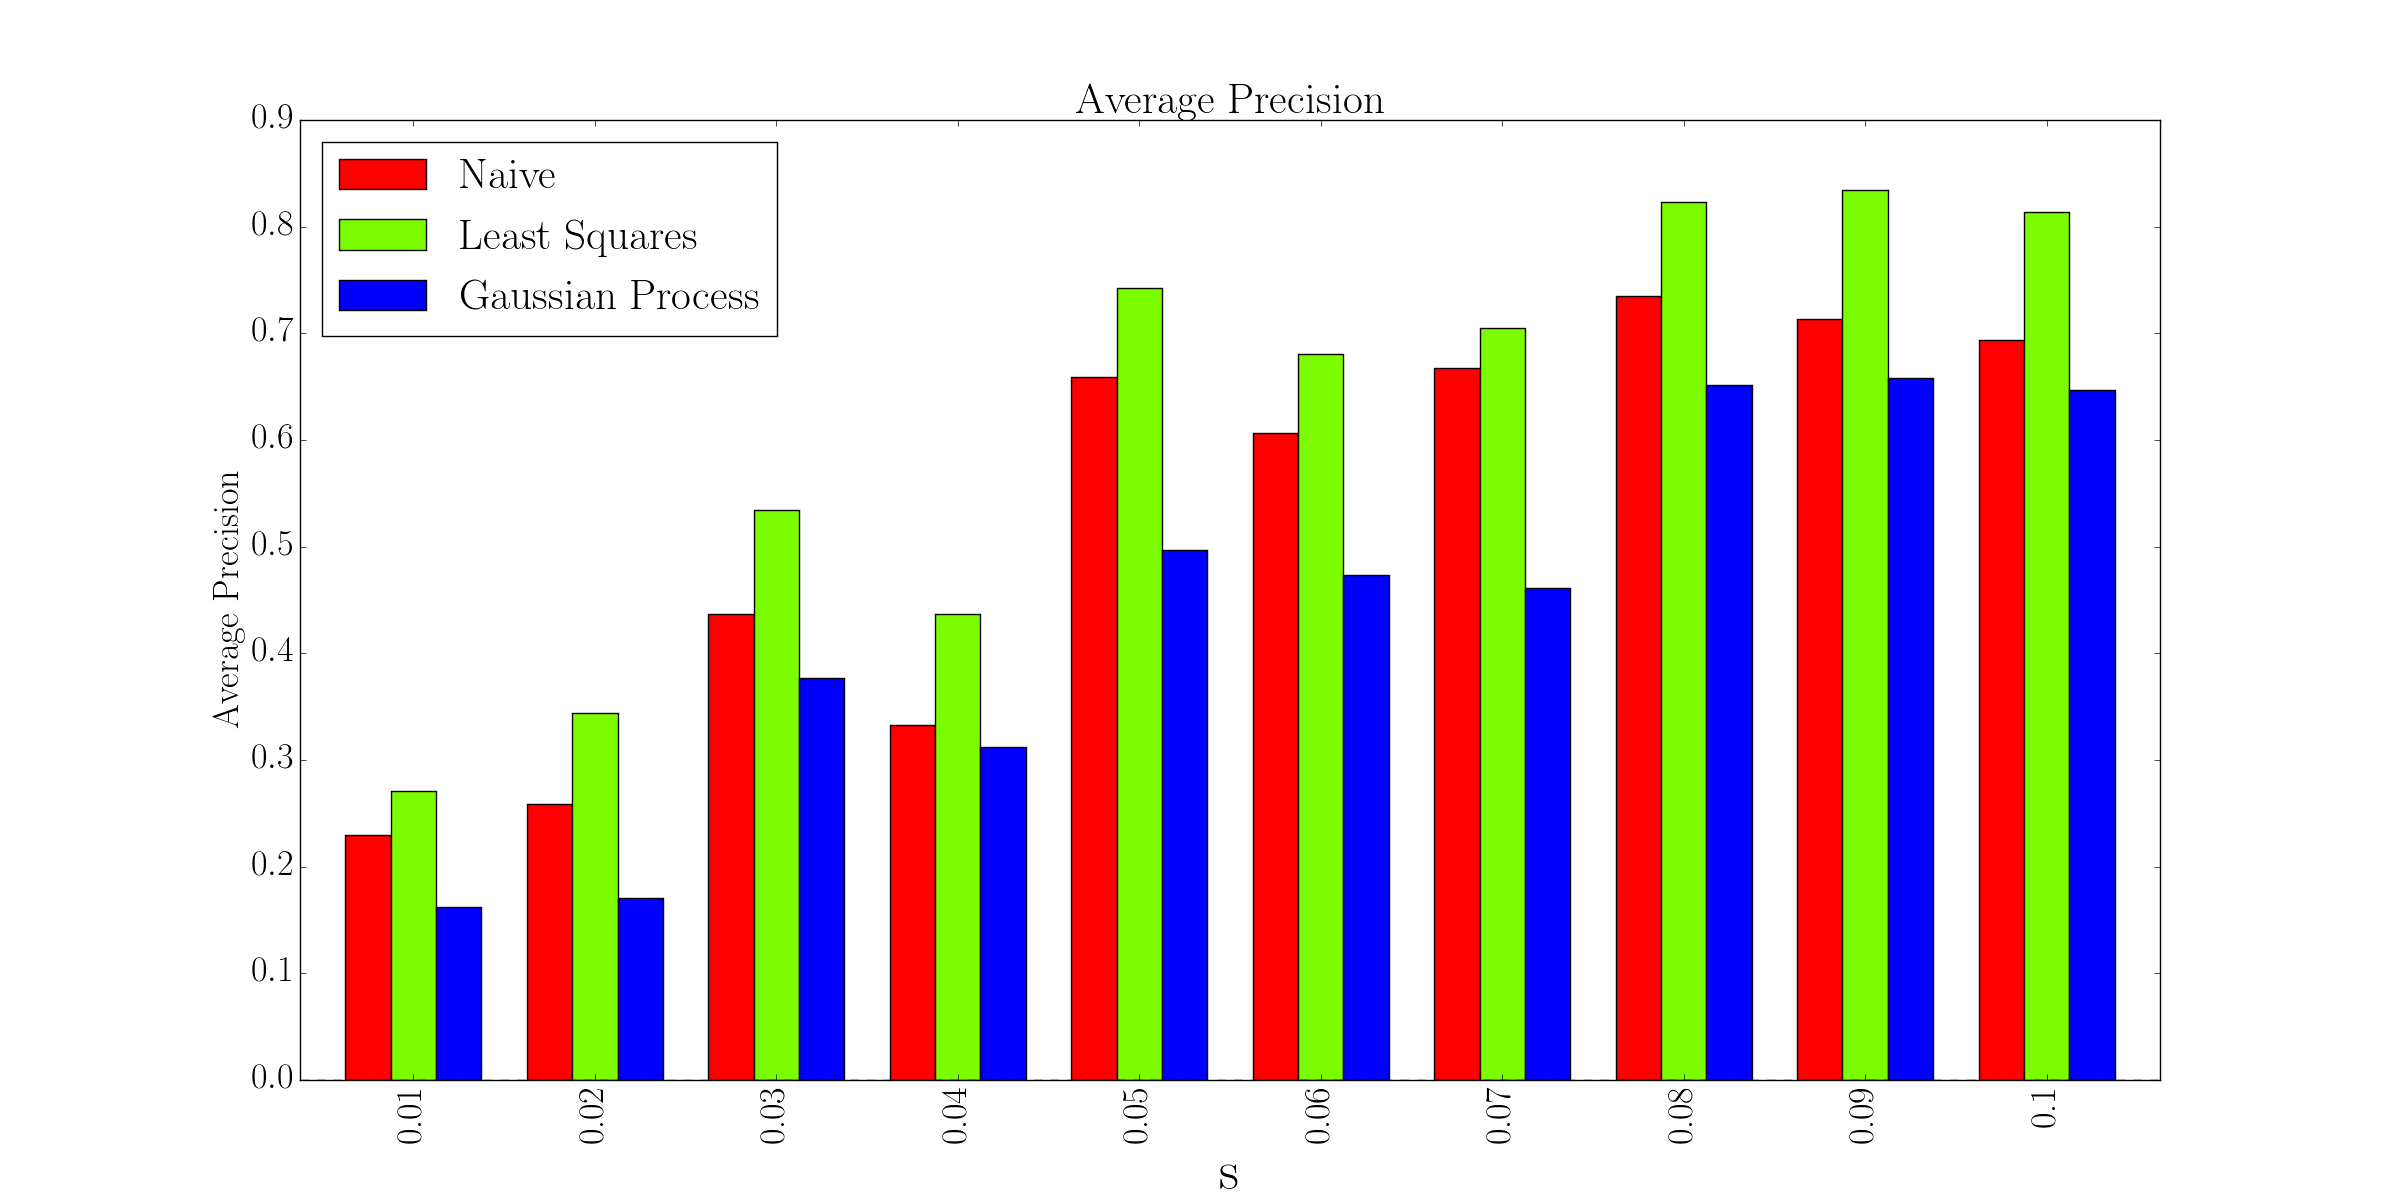
\includegraphics[width=\textwidth]{ap}
  \caption{Mean Average Precision (MAP)}
  \label{fig:Fig5}
\end{figure}


\subsubsection{Estimating Strength of Selection}
\begin{figure}[H]
  \centering
    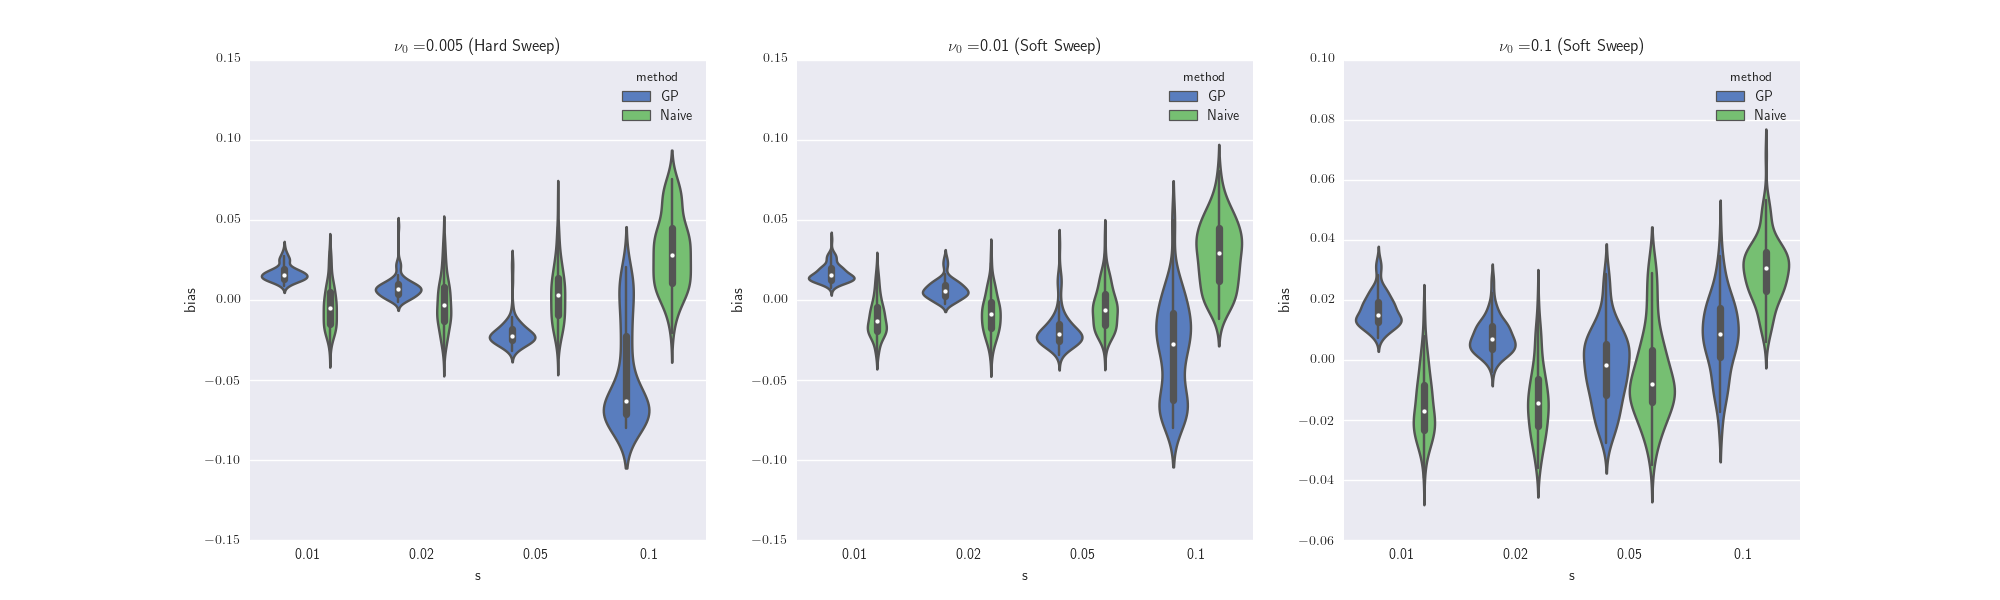
\includegraphics[width=\textwidth]{bias}
  \caption{Bias}
  \label{fig:Fig4}
\end{figure}

\subsection{Computational Performance}
%\section{Discussions}

\newpage
\bibliographystyle{acm}
\bibliography{library}

%%%%%%%%%%%%%%%%%%%%%%%%%%%%%%%%%%%%%%%%%%%%%
%%%%%%%%%%%%%%%%%%% Supplemental Material%%%%
%%%%%%%%%%%%%%%%%%%%%%%%%%%%%%%%%%%%%%%%%%%%%
\clearpage
%\newpage
%\setcounter{page}{1}
\setcounter{figure}{0}
\setcounter{table}{0}
\setcounter{equation}{0}
\renewcommand{\thefigure}{S\arabic{figure}}
\renewcommand{\thetable}{S\arabic{table}}
\renewcommand{\theequation}{S\arabic{equation}}

\section{Appendix}
\subsection{Allele frequencies under selective sweep} \label{app:af}

\beq
\eeq
where $s\in \Rbb$ is the selection coefficient and $o\in[0,1]$ is the 
overdominance parameter which for $u=0.5$ we have
\begin{equation}
x_{t+1}=x_t+\frac{sx_t(1-x_t)}{2+2sx_t}\;.
\label{eq:transition}
\end{equation}
we also have
\beq
\frac{\bfd x_t}{\bfd t} = \frac{sx_t(1-x_t)}{2+2sx_t}
\eeq
which is a differential equation that is difficult to solve. However if take 
the approximation $2+2sx_t \approx 2$, it becomes an ordinary differential 
equation that can be readily solved

\begin{equation}
\nu_t =\frac{1}{1+\frac{1-x_0}{x_0}e^{-st/2}} = \sigma(st/2+\eta(x_0)) 
\label{eq:inf-pop}
\end{equation}
where$\sigma(.)$ is the logistic
function and $\eta(.)$ is logit function (inverse of the logistic function). 

\subsection{Logistic Model for Selection.}
As maximum likelihood for estimating $s$ using Markov chain is computationally 
expensive, here we use and logistic function for modeling allele frequencies 
undergoing selective sweep.
In a pure selection process with no drift, i.e. infinite 
population size, 
dynamic of allele frequencies 
can be well approximated by the logistic function (see 
Appendix \ref{app:af} 
for 
derivation)
\beq
\nu_t=\sigma(st+\eta(\nu_0))\label{eq:nut}
\eeq
where $\sigma(x)=1/(1+e^{-x})$ is the logistic function, and 
$\eta(x)=\log(x)/\log(1-x)$ is inverse of the 
logistic, aka logit, function. Figure \ref{fig:sweep} depicts 
the behavior of 
the logistic model for site allele frequencies and the 
default sampling time 
span(STS). Without genetic drift, soft sweep is easier to 
detect, 
because the logistic function happens to have steeper slope 
in th STS than 
those of hard sweeps, due to standing variation frequency. In addition, even 
under infinite 
population size regime, it is 
difficult differentiate between weak selections and genetic 
drift (a horizontal 
line), in short (e.g. 50 generations) experimental evolutions.


As shown in Figures \ref{fig:dynamic-weak} and \ref{fig:dynamic-strong} (first 
row), the approximate logistic model is consistent with 
simulated data and we 
use it to estimate the strength of selection for 
each site by solving a linear system of equations(see Section 
\ref{sec:regression} for details).

\subsection{Fay Wu's H}\label{app:h}
\bl
In any finite population size of $n$ with $m$ segregating sites, 
allele frequencies take 
discrete values, i.e.,  $x_j \in 
\{\frac{1}{n},\frac{2}{n},\ldots,\frac{n-1}{n}\}, \ \forall j \in{1,\cdot,m}$ 
and we can write
\beq
\|\bfx\|^2= \sum_{j=1}^{m} x_j^2 = 
\sum_{i=1}^{n-1}\left(\frac{i}{n}\right)^2\xi_i= 
\frac{ (n-1)}{2n}H 
\eeq
where $\xi_i$ is the number of sites with frequency $i/n$ and $H$ is the 
Fay \& Wu's estimate of $\theta$.
\el

Recently, Ronen et al. ~\cite{ronen2015predicting} devised the $1\dHAF$ 
statistic for identifying selection on static data, which has the expected 
value related to the $\|\bfx\|^2$:
\begin{equation} 
\Ebb[1\dHAF(t)]= n\| \bfx_t\|^2\approx ng(\nu_t)
\end{equation} 
where
\beq
g(\nu_t)= \theta \nu_t \left(\frac{\nu_t+1}{2} - \frac{1}{(1-\nu_t)n+1}\right) +
\theta (1-\nu_t)\left(\frac{n+1}{2n}-\frac{1}{(1-\nu_t)n+1}\right)
\label{eq:hafscorepooled}
\eeq
where easily follows that
\beq
\theta_H(t)=\frac{n-1}{2} g(\nu_t)
\eeq

\subsection{Tajima's D}\label{app:td}
Let $D_0, \Pi_0, W_0$, be Tajima's D, Tajima's estimate of  $\theta$, and 
Watterson's estimate of $\theta$ at time zero and $D_0=\Pi_0 - W_0$.
In order to compute, $D_t=\Pi_t - W_t$ we compute $\Pi_t$ and $W_t$ separately 
as follows.

Let $P$ be the $n \times n$ matrix of pairwise heterozygosity if individuals, 
then $\Pi=\frac{1}{n^2}\sum P_{ij}$. So, if the population consist of $\nu n$ 
identical carrier haplotype (due to lack of recombination), their pairwise 
hamming distance is zero and should be subtracted from the total $\Pi_t$:
\beq
\Pi_t&= (1-\nu_t^2)\Pi_0 
\eeq

To compute $W_t$, first remember that $W_t= \frac{m_t}{S_n}$ where $m_t$ is the 
number of segregating sites at time $t$ and $S_n= \sum_i^n 1/i \approx 
\log(n)$. Also we have
\beq
\frac{W_t}{W_0}&=\frac{\frac{m_t}{S}}{\frac{m_0}{S}} \ \ \Rightarrow 
W_t=\frac{m_t}{m_0}W0 
\eeq
where $m_t$ to be interpreted as the expected number of segregating sites at 
time $t$, under neutral evolution. At time $t$, the number of individuals that 
undergone neutral evolution is $(1-\nu_t)n +1$, which leads to
\beq
\frac{m_t}{m_0}&=\frac{\log\left((1-\nu_t)n +1 \right)\theta}{\log(n)\theta} 
\approx  
\frac{\log\left((1-\nu_t)n\right)}{\log(n)} = \frac{\log(1-\nu_t)+\log(n)}{\log(n)} = 
1+ \frac{ \log(1-\nu_t)}{\log(n)} 
\eeq
putting all together 
\beq
D_t&= (1-\nu_t^2)\Pi_0 - (1+ \frac{ \log(1-\nu_t)}{\log(n)} ) W_0 = 
D_0-\log(1-\nu_t) \frac{W_0}{\log(n)} -\nu_t^2 \Pi_0
\eeq


\subsection{Linkage Disequilibrium}
Nonrandom associations between polymorphisms are established in the 
substitution process according to the phylogeny, broken by recombination events 
and reinforced by selection. Although in EE the experiments with pooled 
sequencing, LD can not be measured throughout evolution, it is still worthwhile 
to examine the behavior of LD as a result of the interaction between 
recombination and natural selection, to take into account of some of EE 
implicit constraints. 

Let $\rho_0$ be the LD at time zero between the site under selection and a 
segregating site $l$ base-pairs away, then under natural selection we have
\beq
\rho_t= \alpha_t\beta_t \rho_0=e^{-rtl} \left(\frac{H_t}{H0}\right)  
\rho_0\label{eq:ldt}
\eeq
where $H_T=2\nu_0(1-\nu_0)$ is the heterozygousity at the selected site, $r$ is 
the recombination rate/bp/gen. The decay factor $\alpha_t=e^{-rtl}$ is the 
product of recombination and growth factor $\beta_t$ (eq. 30-31 in 
\cite{Stephan2006The})is the outcome of 
selection. For $s=0.01$, $l=100K$bp, the log of decay, growth and product of 
both is depicted in Figure \ref{fig:ldf}. It is evident that, for these 
parameters LD does not start to decay until generation 1000, which would be  
problematic when $\rho_0$. For example, in the case of hard sweep, the 
selection is imposed on the site with minimum AF, which is at perfect linkage 
($|D'|=1$) with all the other loci.\footnote{This is because, between the 
	selected site and all the other sites frequency of one gamete is zero.}
We this phenomenon is shown in the Figures \ref{fig:ld2d}, \ref{fig:ld3d} where 
at generation zero the site at position 500K is at perfect linkage with all the 
other sites, and linkage of the middle site with all the genome is depicted 
for both genetic drift and natural selection, in different generations.
Also, a window of 50Kbp around the selected site is shaded in Figure 
\ref{fig:ld2d} to demonstrate the value of LD in the window under drift and 
hard sweep. This implies that the precision of locating the selection on the 
genome is tightly dependent on a set of parameters including, recombination 
rate, selection strength, initial carrier frequency, and the initial linkage.

\clearpage
\newpage
\section*{Supplemental Figures}



\begin{figure}[H]
	\centering
	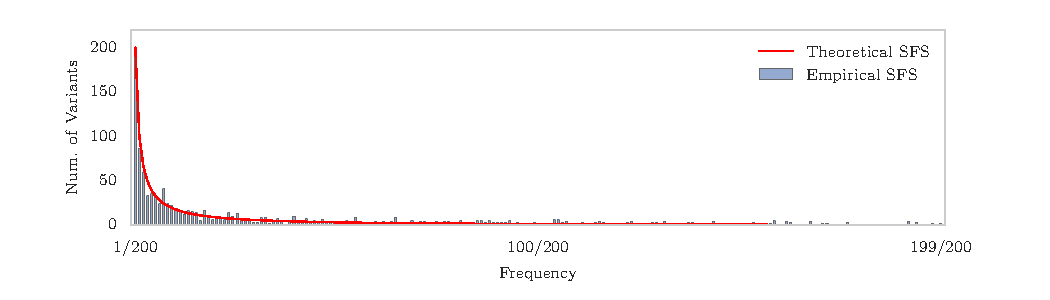
\includegraphics[trim=1in 0.1in 1in 0.1in,clip,width=\textwidth]{figures/sfs.pdf}
	\caption{Theoretical and Empirical SFS for a neutral population of 200 
	individuals.}	\label{fig:sfs}
\end{figure}

\begin{figure}[H]
	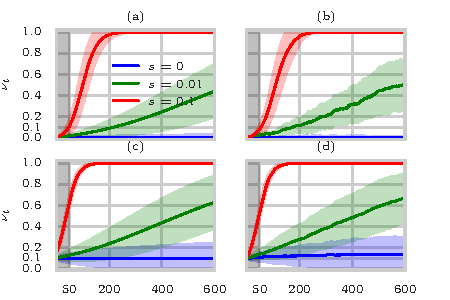
\includegraphics[trim=0in 0.1in 1in 0.1in,clip,width=\textwidth]{figures/AF.pdf}
	\caption{Logistic model for different selection strengths 
		for soft (left) 
		and hard (right) sweep as a function of time in 
		generations. The first 
		50 
		generations, which observations are sampled is 
		shaded.} 	 
	\label{fig:sweep}
\end{figure}
\begin{figure}[H]
	\centering
	\includegraphics[trim={0in 0.1in 0in 
		0in},clip,width=\textwidth]{figures/{tdterms}.png}
	\caption{Interactions of two terms in $D$. W.l.o.g when $D_0=0$ and 
	$\Pi_0=W_0=1$, 
		$D_t$ is sum of the 
		logarithmic $\frac{-\log(1-\nu_t)}{\log(2N)}$ and the squared term 
		$\nu_t^2$.} 	 
	\label{fig:tdterms}
\end{figure}

\begin{figure}[H]
	\centering 
	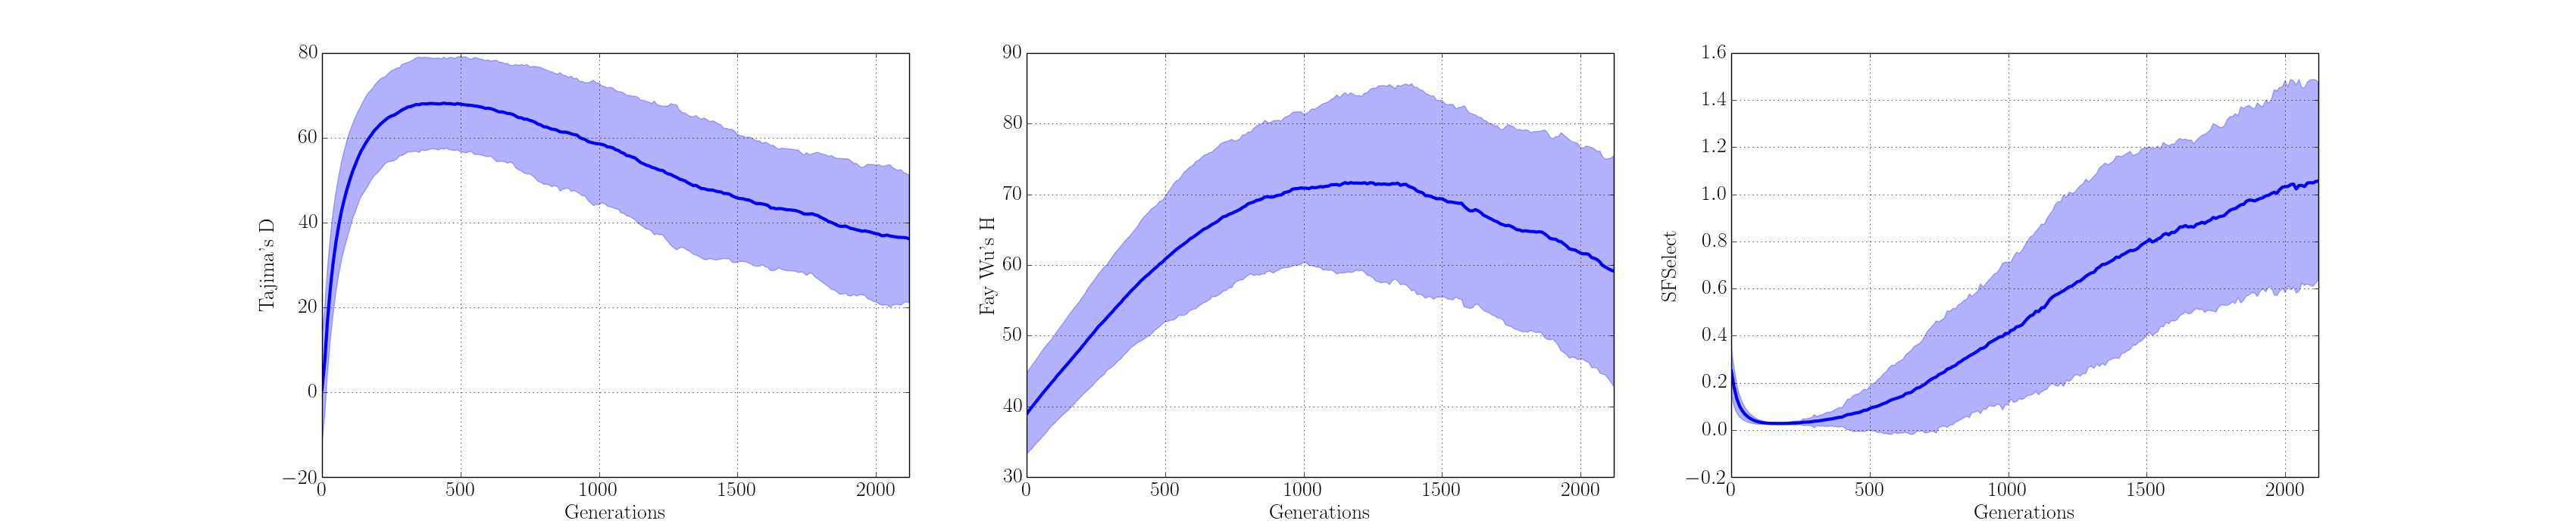
\includegraphics[trim=3.2in 0.1in 3.2in 0.2in , 
	clip,width=\textwidth]{figures/bottleneck}
	\caption{Effect of bottle neck in a typical experimental evoloution 
		experiment where a restricted number of founder lines (here $F=200$) is 
		selected out of a larger population size ($N_e=10^{-6}$). Tajima's D 
		(left), Fay Wu's H (middle) and SFSelect is computed for 1000 neutral 
		simulations and mean and 95\% confidence interval is plotted.} 
	\label{fig:bottleneck}
\end{figure}

\begin{figure}[H]
	\centering 
	\includegraphics[width=\textwidth]{figures/{msmsts}.pdf}
	\caption{Mean and 95\% CI of 1000 simulations for neutral (blue trajectories) selection with $s=0.1$ (red trajectories).}
	\label{fig:sfsts}
\end{figure}



\begin{figure}[H]
	\centering
	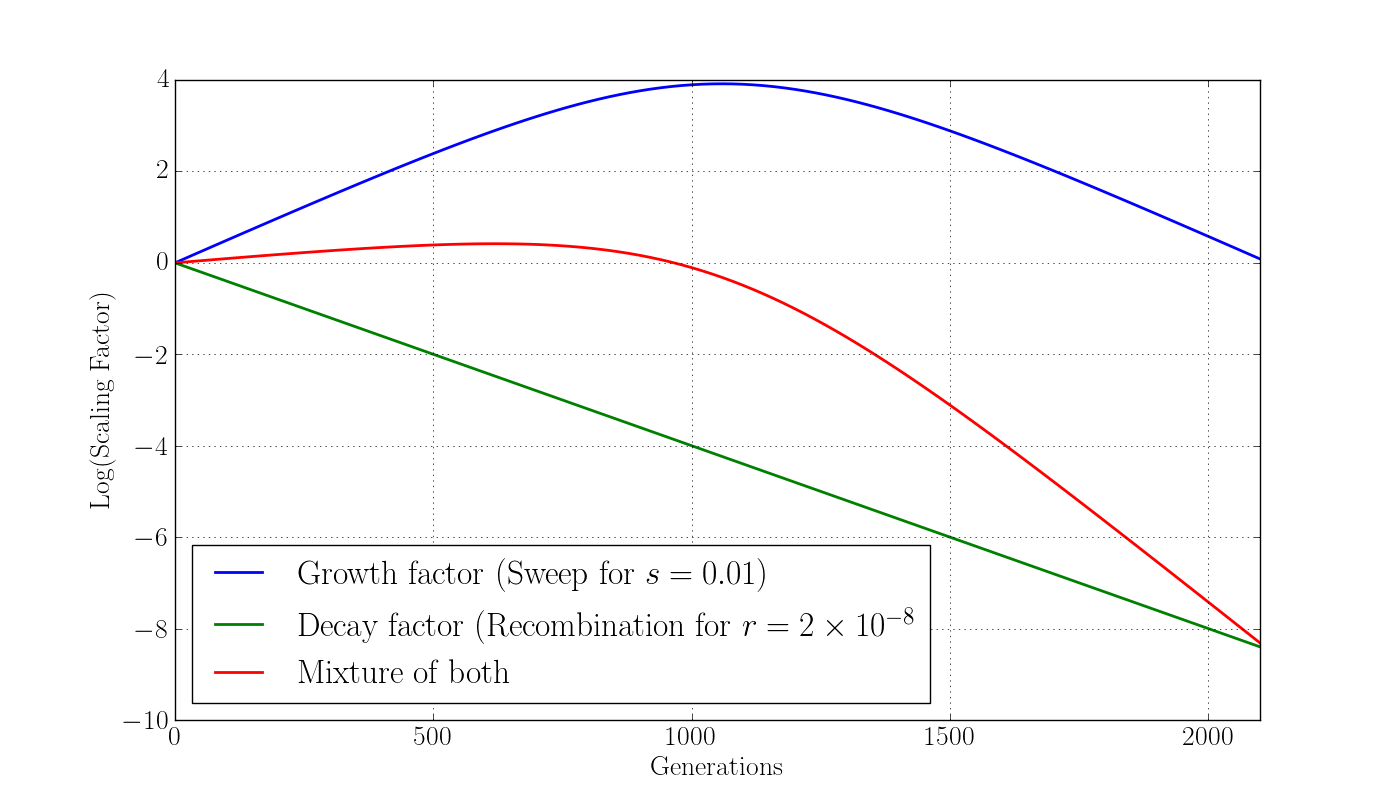
\includegraphics[width=\textwidth]{figures/decayFactors}
	\caption{Interaction between productive factors of LD under natural 
		selection for weak selection (s=$0.01$) and a distance of 100Kb between 
		sites. In this setting, after about 1000 generations LD start to decay 
		(red 
		curve).} \label{fig:ldf}
\end{figure}


\begin{figure}[H]
	\centering
	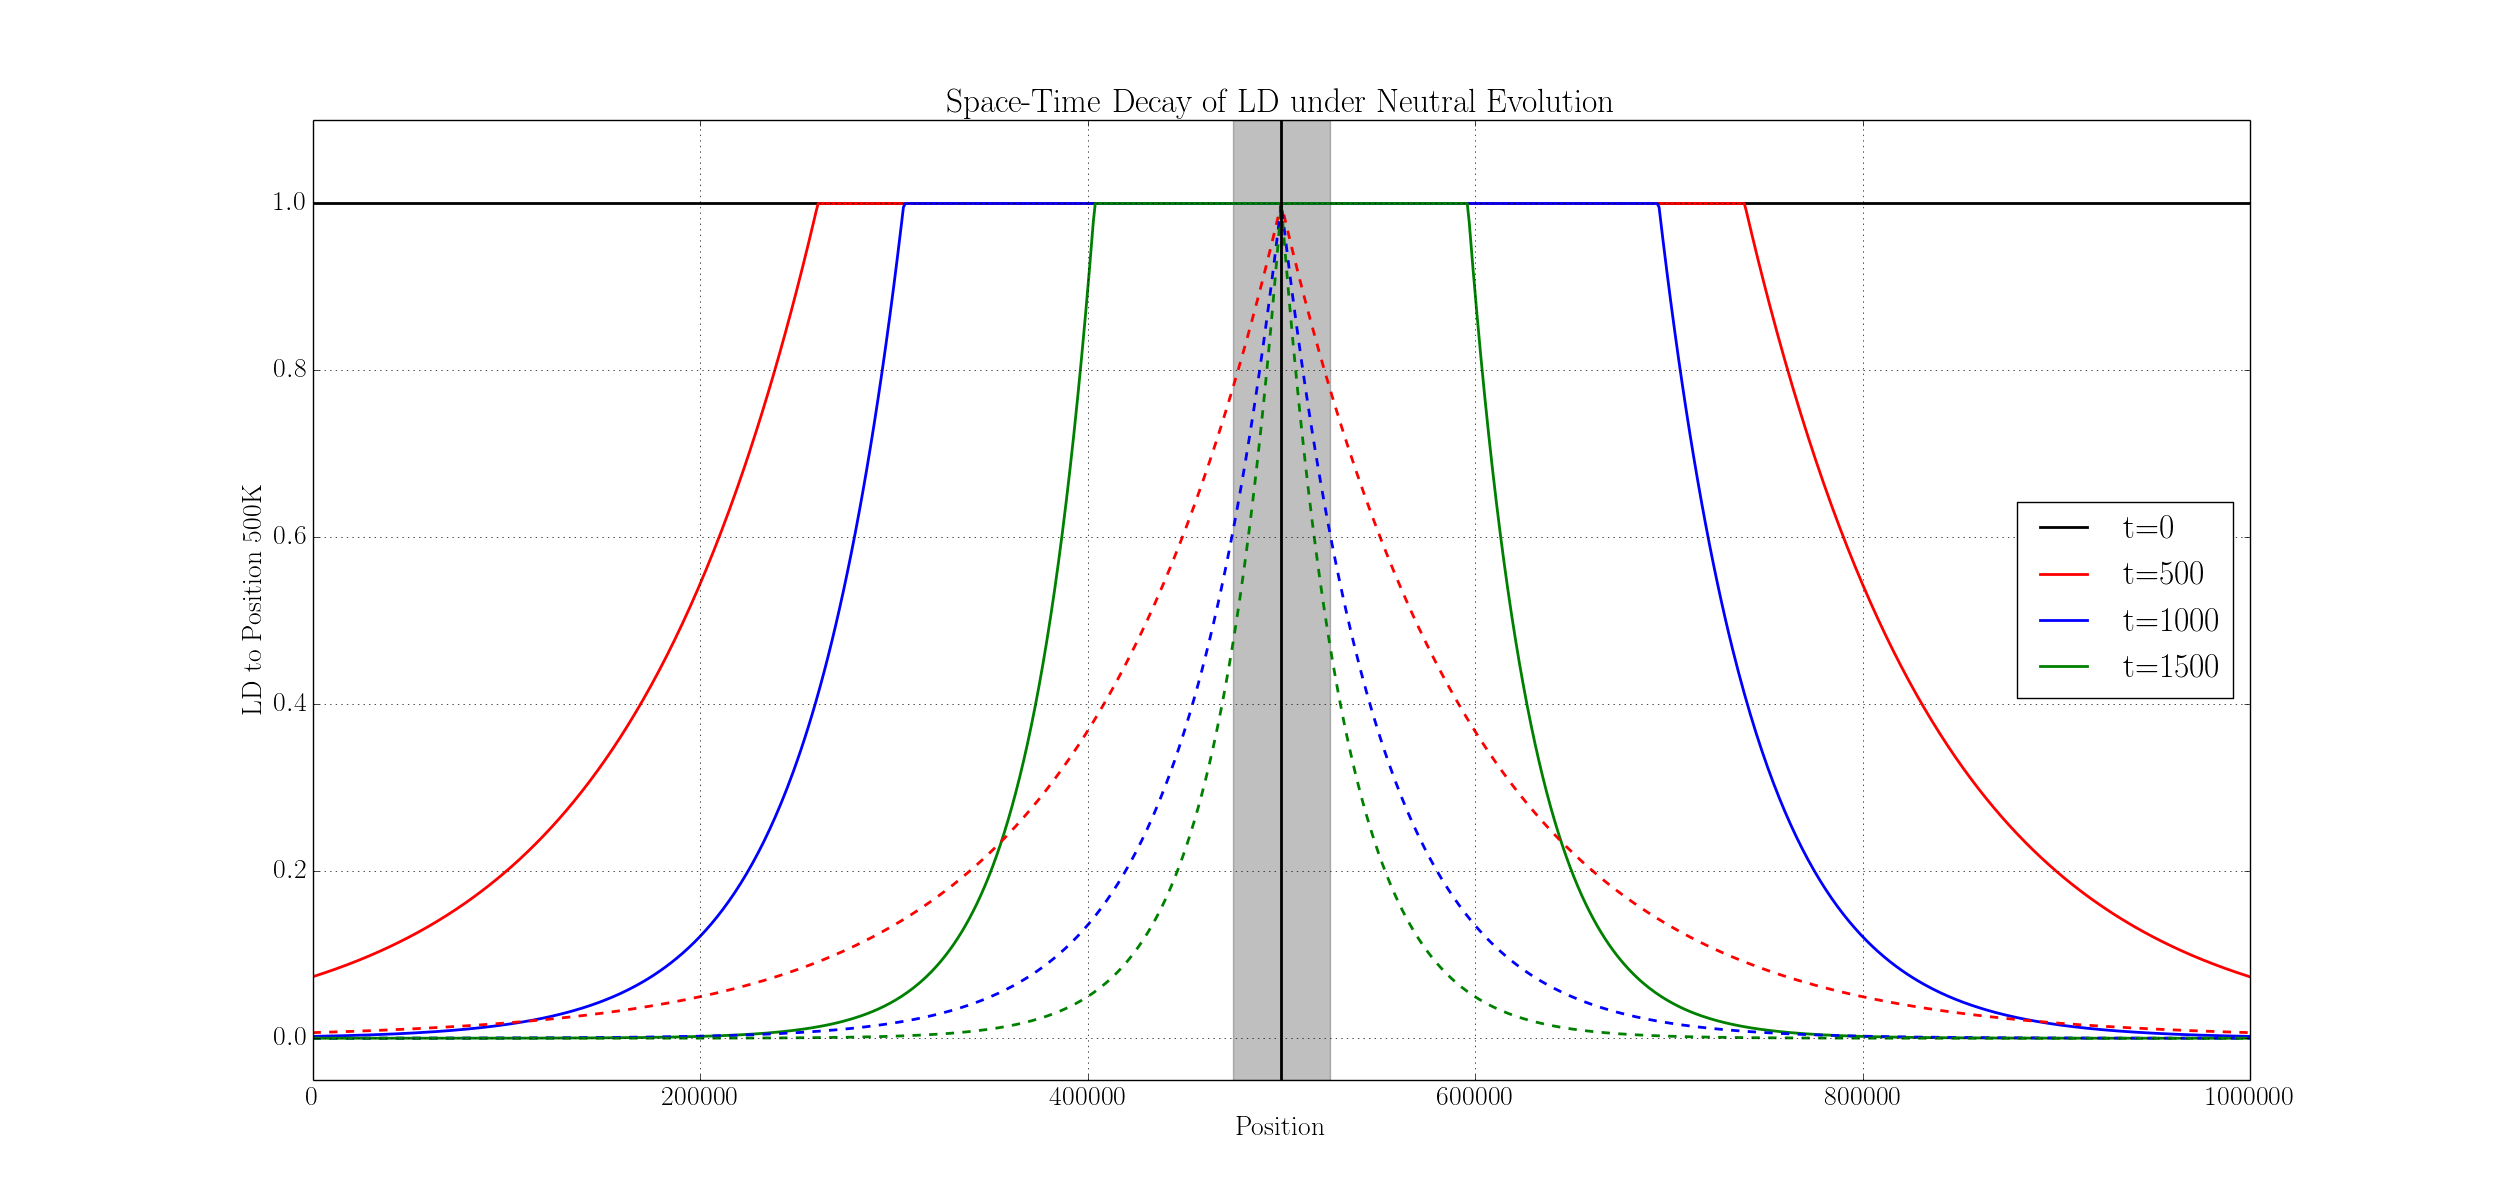
\includegraphics[width=\textwidth]{figures/LDDecay2d}
	\caption{Decay of LD ($|D'|$ measure) of the minimum AF site at position 
		500K with the rest of genome when $s=0.01$ and $r=2\times10^{-8}$. A 
		window 
		of 50Kb is shaded at the center of genome to illustrate high values of 
		linkage in both selection and drift.} \label{fig:ld2d}
\end{figure}


\begin{figure}[H]
	\centering
	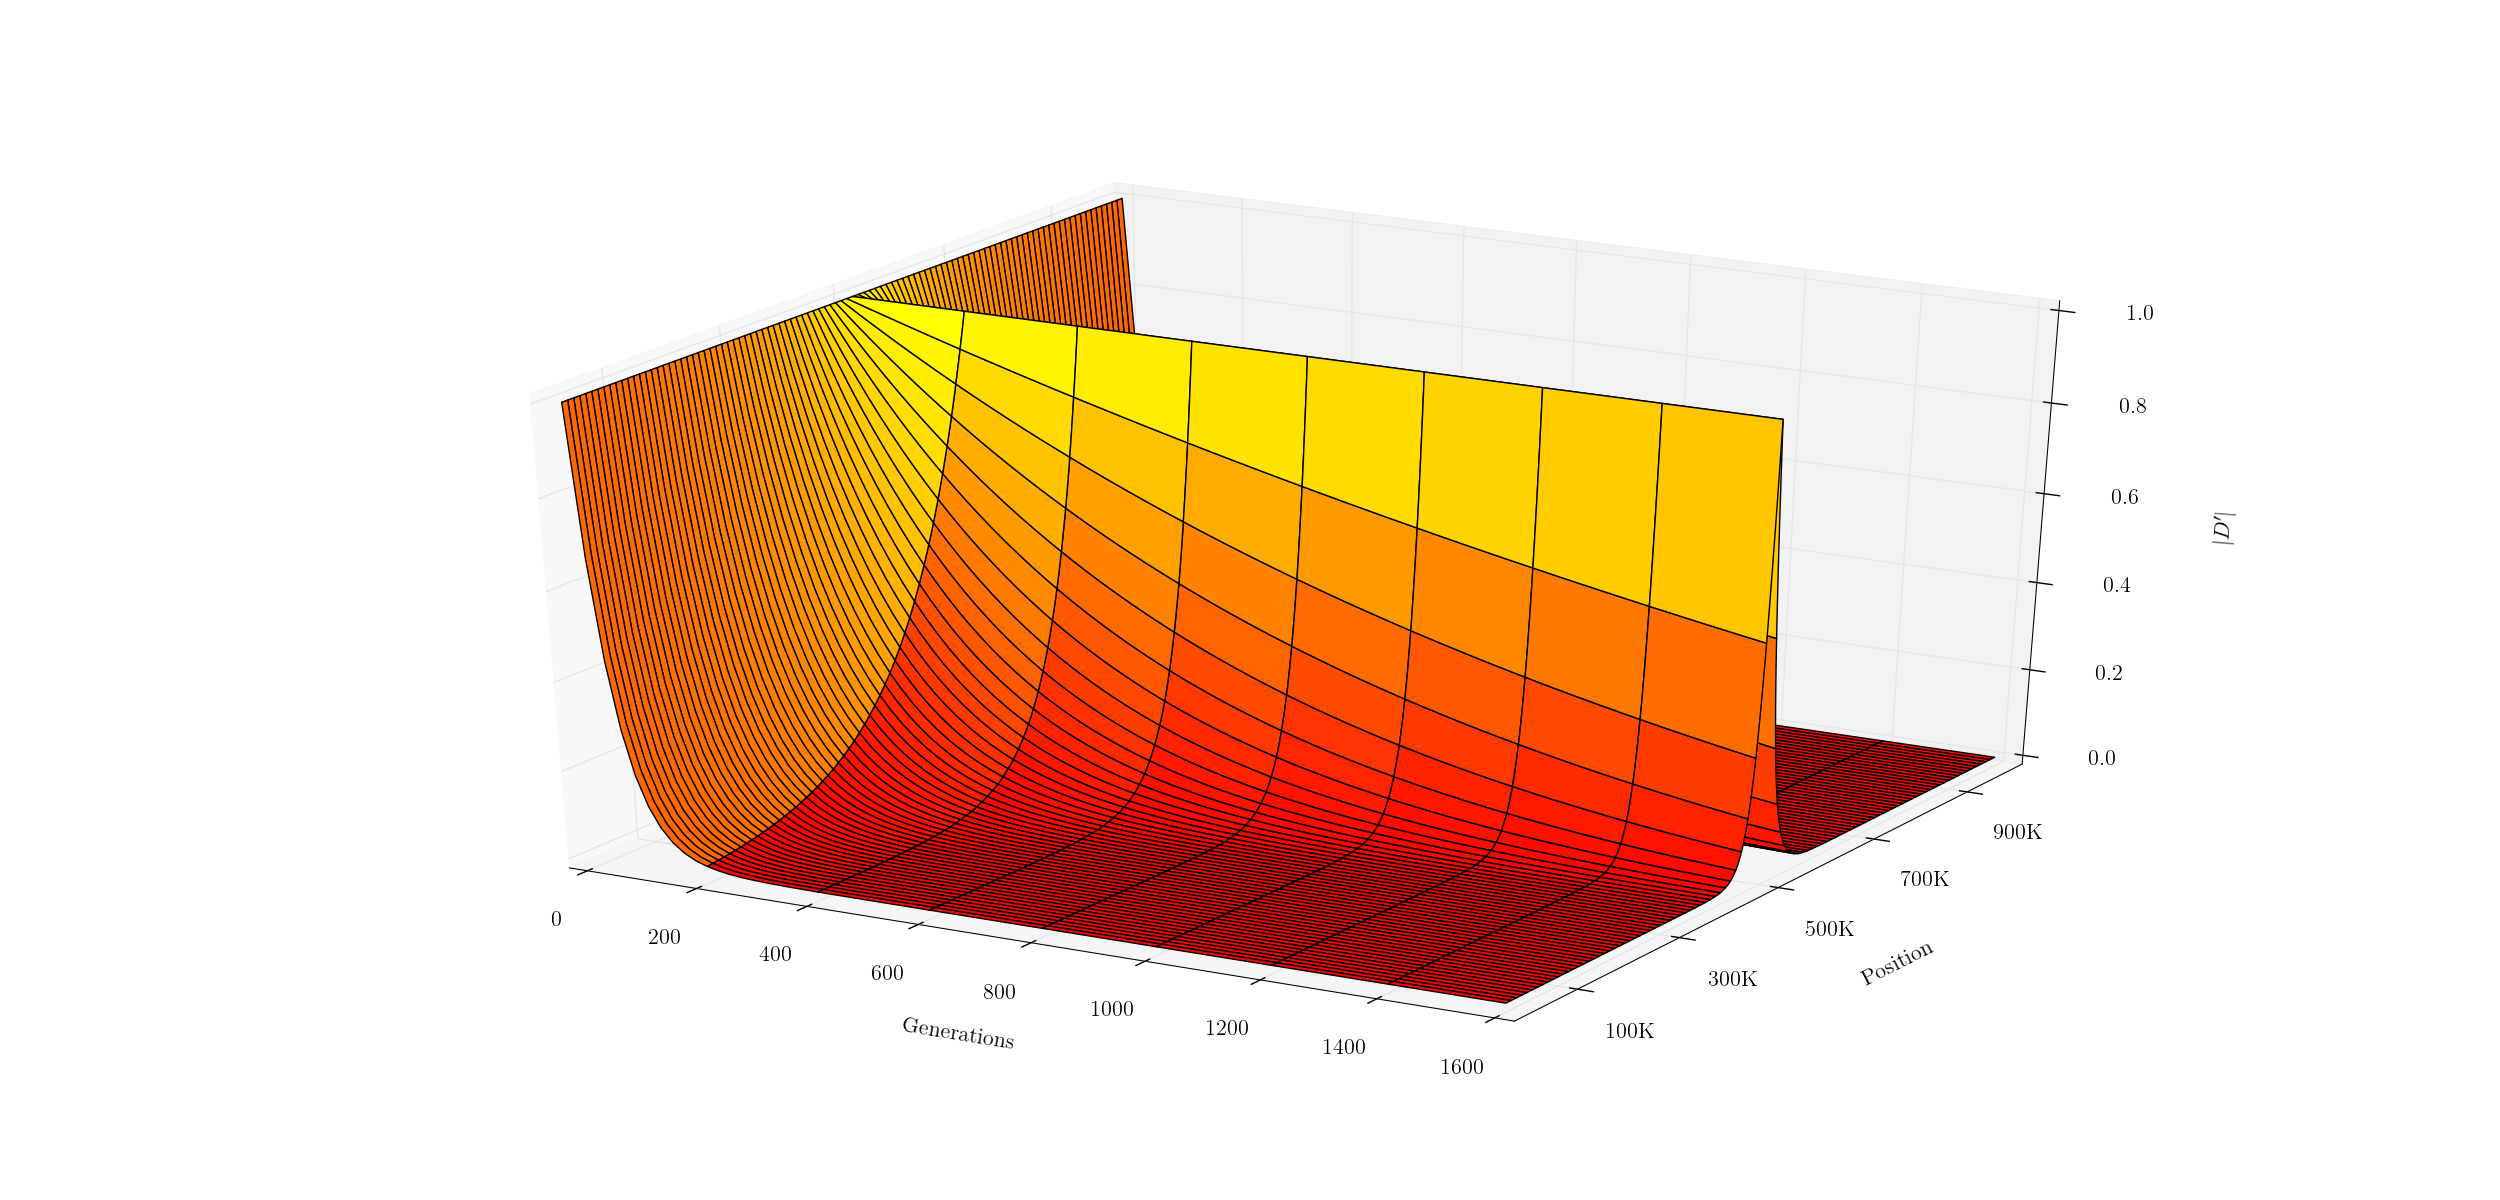
\includegraphics[width=\textwidth]{figures/LDDecay3dNeutral}
	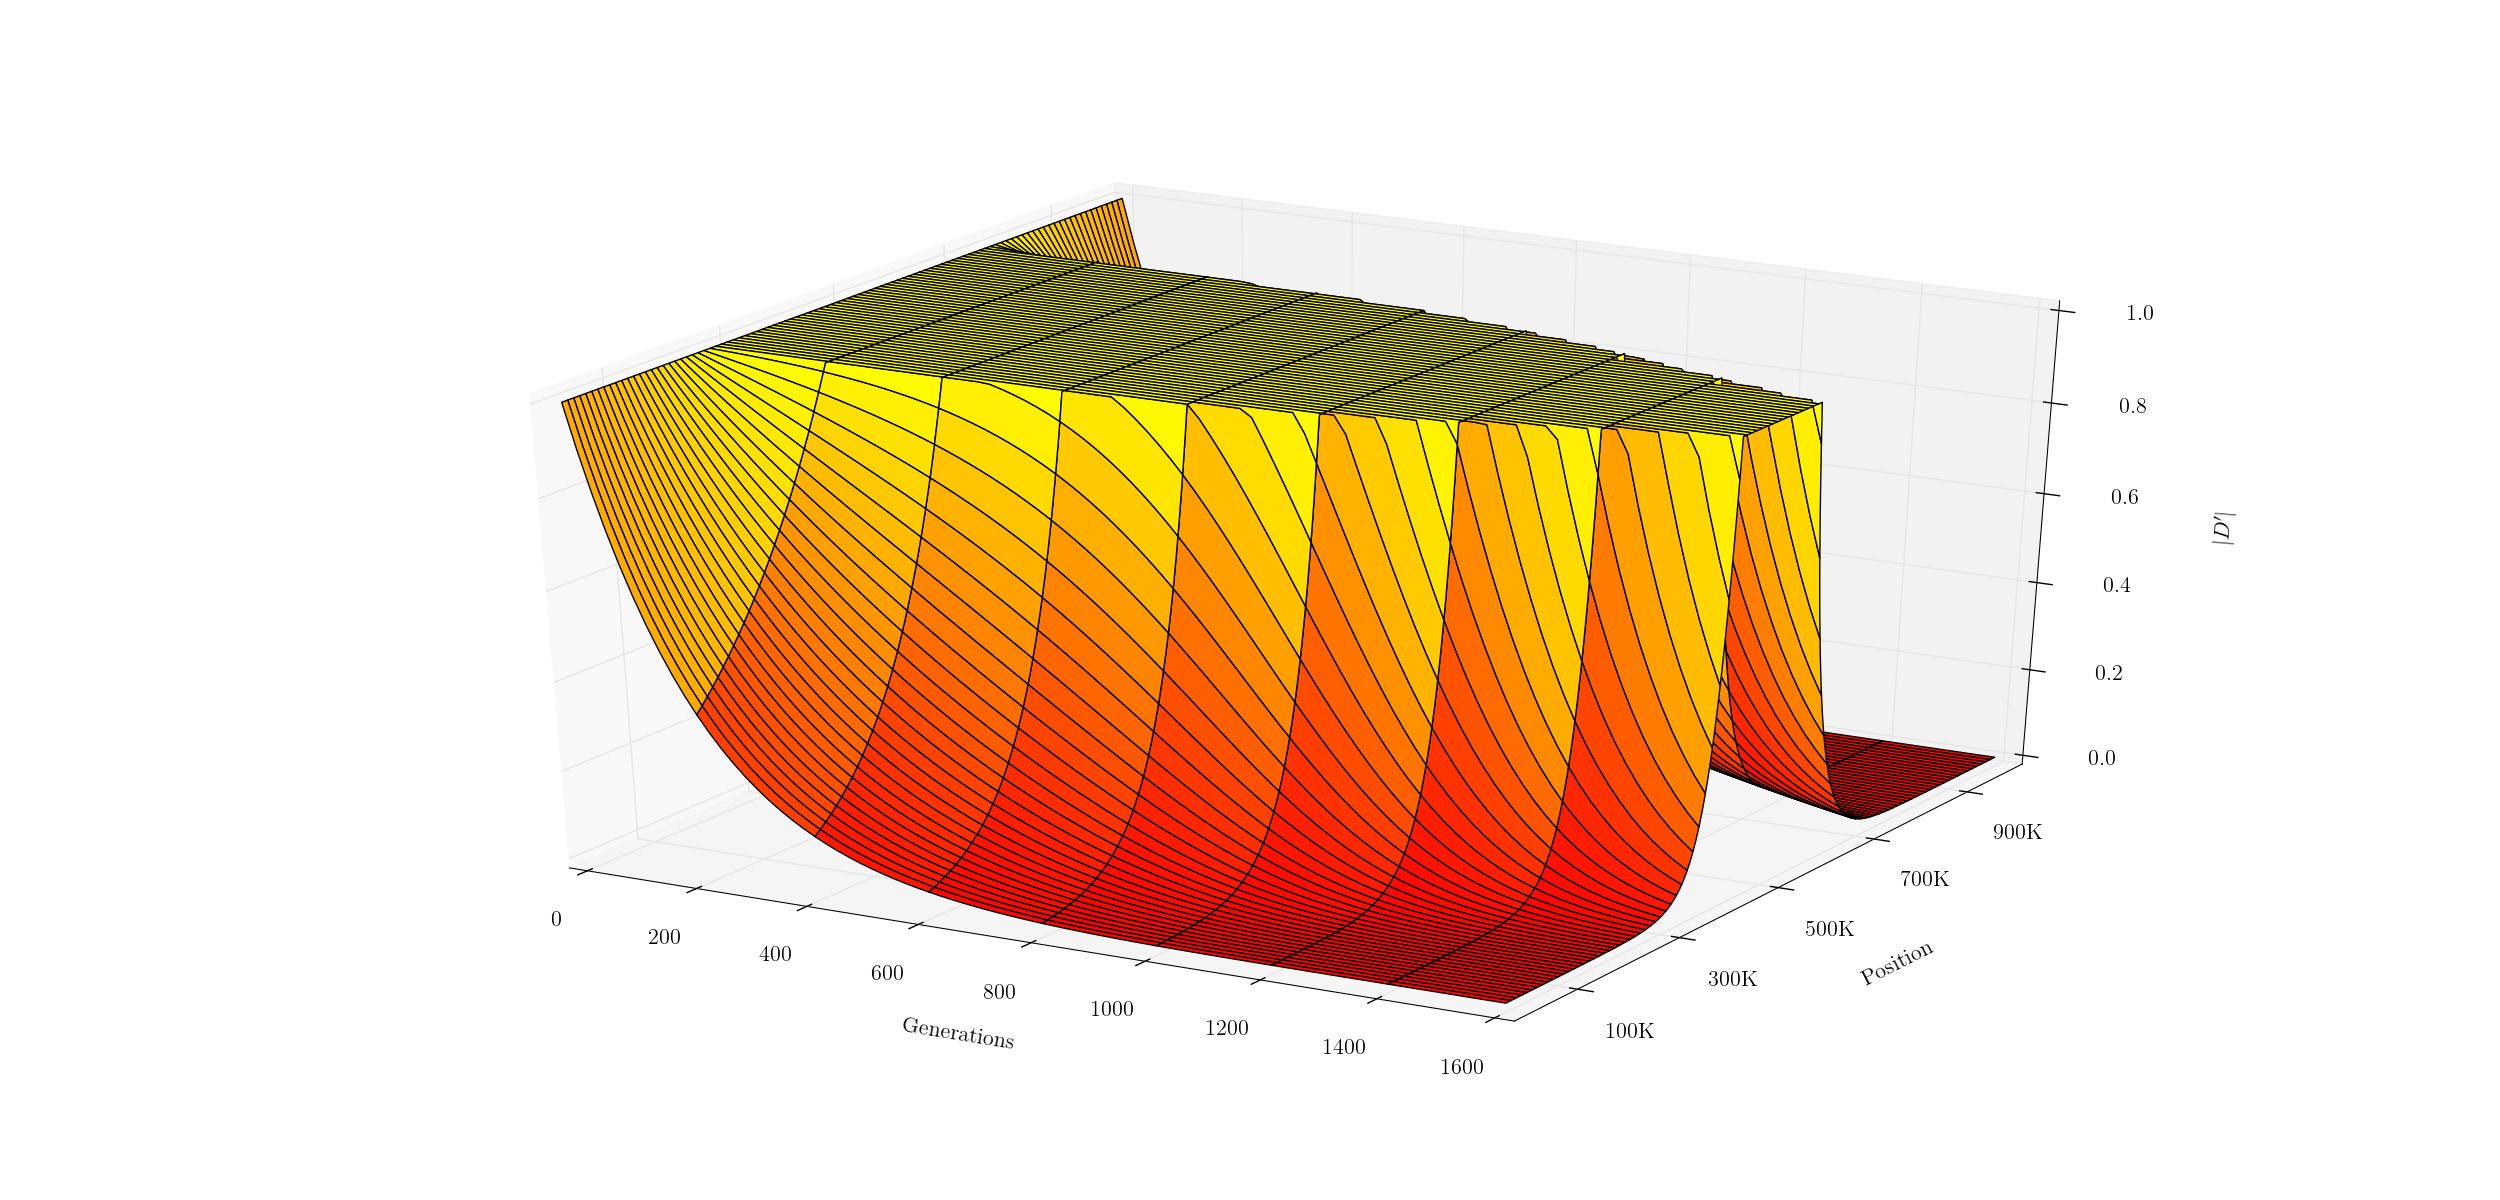
\includegraphics[width=\textwidth]{figures/LDDecay3dSweep}
	\caption{ld} \label{fig:ld3d}
	\caption{Decay of LD ($|D'|$ measure) of the minimum AF site at 
		position 500K with the rest of genome in genetic drift with 
		$r=2\times10^{-8}$ (top) and hard sweep with $s=0.01$ (bottom).}
\end{figure}




\begin{figure}[H]
	\centering
	\includegraphics[trim=1.2in 0 .0in 0, 
	clip,width=\textwidth]{figures/{dominance}.png}
	\caption{Dominance for $s=0.1$.} 
	\label{fig:dominance}
\end{figure}

\begin{figure}[H]
	\centering
	\includegraphics[trim=.2in 0 .0in 0, 
	clip,width=\textwidth]{figures/{qq}.pdf}
	\caption{QQ plot for a simulation.} 
	\label{fig:qq}
\end{figure}

\begin{figure}[H]
	\centering
	\includegraphics[trim=.2in 0 .0in 0, 
	clip,width=\textwidth]{figures/{stab}.pdf}
	\caption{100$^{th}$ power of the transition matrix for neutral (left) and selection with $s=0.1$ (right).} 
	\label{fig:qq}
\end{figure}

\begin{figure}[H]
	\centering
	\includegraphics[trim=.2in 0 .0in 0, 
	clip,width=\textwidth]{figures/{stab}.pdf}
	\caption{100$^{th}$ power of the transition matrix for neutral (left) and selection with $s=0.1$ (right).} 
	\label{fig:qq}
\end{figure}

\begin{figure}[H]
	\centering
	\includegraphics[trim=.0in 0 .0in 0, 
	clip,width=\textwidth]{figures/{samplingTimes}.pdf}
	\caption{sampling times.} 
	\label{fig:nullpred}
\end{figure}


\begin{figure}[H]
	\centering
	\includegraphics[trim=.2in 0 .0in 0, 
	clip,width=\textwidth]{figures/{candidateSNPDensity}.pdf}
	\caption{Density.} 
	\label{fig:nullpred}
\end{figure}

\begin{figure}[H]
	\centering
	\includegraphics[trim=.0in 0 .0in 0, 
	clip,width=\textwidth]{figures/{stateConditional}.pdf}
	\caption{observation state transition.} 
	\label{fig:nullpred}
\end{figure}

\begin{figure}[H]
	\centering
	\includegraphics[trim=.2in 0 .0in 0, 
	clip,width=\textwidth]{figures/{nullpred}.pdf}
	\caption{Empirical null distribution of test statistic on 1M simulations.} 
	\label{fig:nullpred}
\end{figure}



\begin{figure}[H]
	\centering
	\begin{tabular}{cc}
			\includegraphics[trim=.2in 0 .0in 0, 
			clip,width=0.5\textwidth]{figures/{nulls}.pdf}
			&\includegraphics[trim=.2in 0 .0in 0, 
			clip,width=0.5\textwidth]{figures/{nulls.log}.pdf}
	\end{tabular}
	\caption{Empirical null distribution of $s$ statistic on 1M simulations.} 
	\label{fig:nullpred}
\end{figure}



\begin{figure}[H]
	\centering
	\begin{tabular}{c}
				\includegraphics[trim=.2in 0 .0in 0, 
				clip,width=\textwidth]{figures/{HSP}.pdf}\\
		\includegraphics[trim=.2in 0 .0in 0, 
		clip,width=\textwidth]{figures/{BM}.pdf}\\
		\includegraphics[trim=.2in 0 .0in 0, 
		clip,width=\textwidth]{figures/{BF}.pdf}\\
	\end{tabular}
	\caption{Song, HSF, HSP.} 
	\label{fig:nullpred}
\end{figure}


\begin{figure}[H]
	\centering
	\begin{tabular}{c}
		\includegraphics[trim=.2in 0 .0in 0, 
		clip,width=\textwidth]{figures/{depth}.pdf}
	\end{tabular}
	\caption{Scaled PDF (left) and CDF (right) of the overall read depth distribution (top) and minimum depth of sites (bottom).
		Top row depicts the overall distribution of rad of all reads.} 
	\label{fig:depth}
\end{figure}

\begin{figure}[H]
	\centering
	\begin{tabular}{c}
		\includegraphics[trim=.2in 0 .0in 0, 
		clip,width=\textwidth]{figures/{depthHetero}.pdf}
	\end{tabular}
	\caption{Read depth at four different sites. (which would be filtered if the min depth is set to 30X)} 
	\label{fig:depthHetero}
\end{figure}

\begin{figure}[H]
	\centering
	\begin{tabular}{c}
		\includegraphics[trim=.2in 0 .0in 0, 
		clip,width=\textwidth]{figures/{siteDepthDist}.pdf}\\
	\end{tabular}
	\caption{Distribution of the mean and variance of the minimum depth of all sites.} 
	\label{fig:siteDepthDist}
\end{figure}
\begin{figure}[H]
	\centering
	\begin{tabular}{c}
		\includegraphics[trim=.2in 0 .0in 0, 
		clip,width=\textwidth]{figures/{probS}.pdf}\\
	\end{tabular}
	\caption{Empirical conditional distribution of $s$.} 
	\label{fig:probS}
\end{figure}
\newpage
\bibliographystyle{acm}
\bibliography{library}

\end{document}
